\documentclass[11pt]{article}

\usepackage[utf8]{inputenc}
\usepackage{amsmath, amssymb, amsthm}
\usepackage[inkscapeformat=pdf]{svg}
\usepackage{placeins}
\usepackage{tabularx}
\usepackage{float}
\usepackage{setspace}
\usepackage{hyperref}
\usepackage{enumitem}
\usepackage{parskip}
\usepackage{ffcode}
\usepackage{graphicx}
\usepackage{caption}

\usepackage[margin=2cm]{geometry}

\def\code#1{{\texttt{#1}}}

\title{%
  \textbf{DD} \\
  \large Software Engineering Project \\ A.Y. 2022-2023}

\author{Marco Ronzani, Alessandro Sassi}

\date{December 2022}

\begin{document}

\maketitle

\doublespacing
\tableofcontents
\singlespacing

\section{Introduction}
\label{section:introduction}

\subsection{Purpose}

Electric vehicles are starting to grow in number, and their takeover of combustion engines is bound to happen, consequently to support such a thriving trend adequate easy access to charging stations is of utmost importance. In this landscape the goal of eMall is to allow owners of electric vehicles to easily know where charging stations are and carefully plan their charging process according to their schedules at any such station. \\
\\
This document will follow up on the RASD document with a discussion of the architectural design of the system, its main architectural components and their interfaces. It will also cover the plans for implementation and integration, as well as those for testing, with the goal of guiding the development process. \\

\subsection{Scope}

This DD document takes into consideration the requirements and specifications of the eMSP platform “eMall”, together with its interaction with one or more CPMSs. The stakeholders considered are the End Users who interact with the “eMall” platform, CPOs owning the respective CSs and CPMSs, and DSOs offering their services to the aforementioned parties.

\subsection{Definitions, Acronyms and Abbreviations}

\subsubsection{Definitions}

\begin{table}[H]
    \centering
    %space between text and right/left borders
    \setlength{\tabcolsep}{18pt}
    %Row height multiplier
    \renewcommand{\arraystretch}{1.2}
    \begin{tabularx}{\textwidth}{|>{\centering\hsize=0.4\hsize}X|>{\hsize=1.6\hsize}X|}
        \hline
        \textbf{Term} & \textbf{Definition} \\
        \hline
        Charging Station & Device with a connection to the electric grid which brakes out power to one or more socket(s) for vehicles. Monitoring of each socket's status. \\
        \hline
        Socket & One of the charging outlets available at a CS where a vehicle connects, its type determines the vehicles that can connect. \\
        \hline
        Charging Session & The process in which a User performs a recharge of their vehicle at a specific socket. \\
        \hline
        Energy source of a Charging Station & Batteries or the DSO currently assigned to the CS, whichever the CS is currently drawing its power from. \\
        \hline
        Charging Station External Status & Number of charging sockets available, their type such as slow/fast/rapid, their cost, and, if all sockets of a certain type are occupied, the estimated amount of time until the first socket of that type is freed. \\
        \hline
        Charging Station Internal Status & Amount of energy available in the batteries, if any, number of vehicles being charged and, for each charging vehicle, amount of power absorbed and time left to the end of the recharge. \\
        \hline
        Energy Source & Method of energy production that results in a known fraction of the energy supplied to an endpoint in the electric grip. \\
        \hline
        User-price & Cost of a recharge that is shown to the User when they inspect a CS and is what they are charged for. It is set by the CPO/CPMS on a per-CS basis.\\
        \hline
        Nominal-price & Cost of a recharge at a CS without any discount or offer applied, it is set by the CPO/CPMS on a per-CS basis. A user-price $<$ nominal-price implies an ongoing special offer. \\
        \hline
        Energy source management policy OR Battery usage policy & A per-CS policy given them by the CPMS to allow them to dynamically decide whether to acquire energy from their assigned DSO or from their batteries and when to charge their batteries with energy from their DSO. \\
        \hline
        Charge Point Management System's policy for “Automatic Mode” & The global policy used by the CPMS to operate autonomously, its mainly built around thresholds and weights to allow the CPMS to decide prices and battery usage policies for its CSs. \\
        \hline
        Offer reset date & The date, set on a per-CS basis, at which a CS will reset its user-price to the value of its nominal-price, removing any present offer. \\
        \hline
    \end{tabularx}
    \label{tab:definitions}
\end{table}

\subsubsection{Acronyms}

\begin{table}[H]
    \centering
    %space between text and right/left borders
    \setlength{\tabcolsep}{18pt}
    %Row height multiplier
    \renewcommand{\arraystretch}{1.2}
    \begin{tabularx}{\textwidth}{|>{\centering\hsize=0.3\hsize}X|>{\hsize=1.7\hsize}X|}
        \hline
        \textbf{Acronym} & \textbf{Full Name} \\
        \hline
        eMall & Electric Mobility for All \\
        \hline
        eMSP & Electric Mobility Service Provider \\
        \hline
        CPO & Charging Point Operator \\
        \hline
        CPMS & Charge Point Management System \\
        \hline
        CS & Charging Station \\
        \hline
        DSO & Distribution System Operator \\
        \hline
        STB & System-To-Be \\
        \hline
        OS & Operating system \\
        \hline
        DB & Database \\
        \hline
    \end{tabularx}
    \label{tab:acronyms}
\end{table}

\subsection{Revision History}

\begin{enumerate}
    \item[v0.1] First draft of the document.
\end{enumerate}

\subsection{Reference Documents}

\begin{enumerate}
    \item The provided document describing the project: \textit{Assignment RDD AY 2022-2023-v3}.
    \item The Software Engineering 2 course held by Prof.s Camilli Matteo, Di Nitto Elisabetta and Rossi Matteo Giovanni.
    \item \textit{ISO/IEC/IEEE 29148:2011(E)} standard for Requirement Engineering.
    \item Project of last year provided as an assignment.
\end{enumerate}

\subsection{Document Structure}

The document is divided into the following N sections.

The \textbf{architecture design} introduces the structure of the STB and its main components in regard to both the eMSP and the CPMS. Every component is thoughtfully described in its purpose and position in the components hierarchy. Following the components description in a view of how the STB will be deployed and its runtime interactions between the various components of across both the eMSP and CPMS. In the subsection the main design decision behind the system architecture are elicitated and discussed in futher details. \\
\\
The \textbf{user interface design} section resumes what was already present in the RASD document and futher expands on it. \\
\\
The \textbf{implementation, integration and test plan} section then proceeds to discuss how the architecture previously described will be realized, with its modules integrated and tested in order to guarantee the correctness of the final product, w.r.t. the requirements and directions expressed both in this document and the RASD, during each step of development. \\
\\
The \textbf{effort spent} section presents data regarding the amount of time each team member invested in the creation of this document. \\
\\
Finally \textbf{references} are reported.

\newpage

\section{Architectural Design}

%For now considering: Express (NodeJs) + MySQL/Postgre

%4-tier architecture (places where layers are deployed) both for eMSP and CPMS:
% >Presentation/Client
% >Web Server
% >App Server
% >DB Server

%Architettura monolitica, vecchio stile
%Giustificazione: la abbiamo progettata così che sia facilmente divisibile in microservice qualora il carico sul sisteme richedesse la distribuzione delle funzionalità su più macchine. Inoltre i benefici alla sicurezza di avera un sistema monolitico non sono trascurabili.

%4-layer to map over the physical entities (not 1:1 necessarily)
%http://www.hanselman.com/blog/a-reminder-on-threemulti-tierlayer-architecturedesign-brought-to-you-by-my-late-night-frustrations
% >Presentation
% >Business logic
% >Data Access
% >Data Store

%Server 1: eMSP + DB
%Server 2: CPMS + DB

%CS client del CPMS

\subsection{Overview}

The system architecture can be split into 2 main parts: one for the eMSP, the other one for the CPMS. \\
The eMSP adopts an architecture organized into \textbf{four layers} distributed over \textbf{four tiers}, resulting in a monolithic structure with benefits for security and maintenance, given that there are less entry points for possible attack vectors. This monolityic architecture is also quite appropriate for the system-to-be, since the services it needs to provide are all closely related. However, it should be noted that its modular approach would allow for an easy transition to microservices when, if ever, the load imposed on the system will require the distribution of its functionalities over multiple machines. Therefore, the eMSP system is composed of a \textbf{presentation layer}, running the client-side application, a \textbf{Web Server} and \textbf{Application Server} to handle API routing and web app page serving, and finally a \textbf{dedicated DB Server}. \\
The CPMS adopts an analogous architectural pattern, with the same \textbf{four layers} and \textbf{four tiers}. However, in order to communicate with the CSs it owns, they are modeled as clients, which run a custom application and communicate with the CPMS platform through the Web Server and its exposed APIs. \\

%trim = left bottom right top
\begin{figure}[!ht]
    \centering
    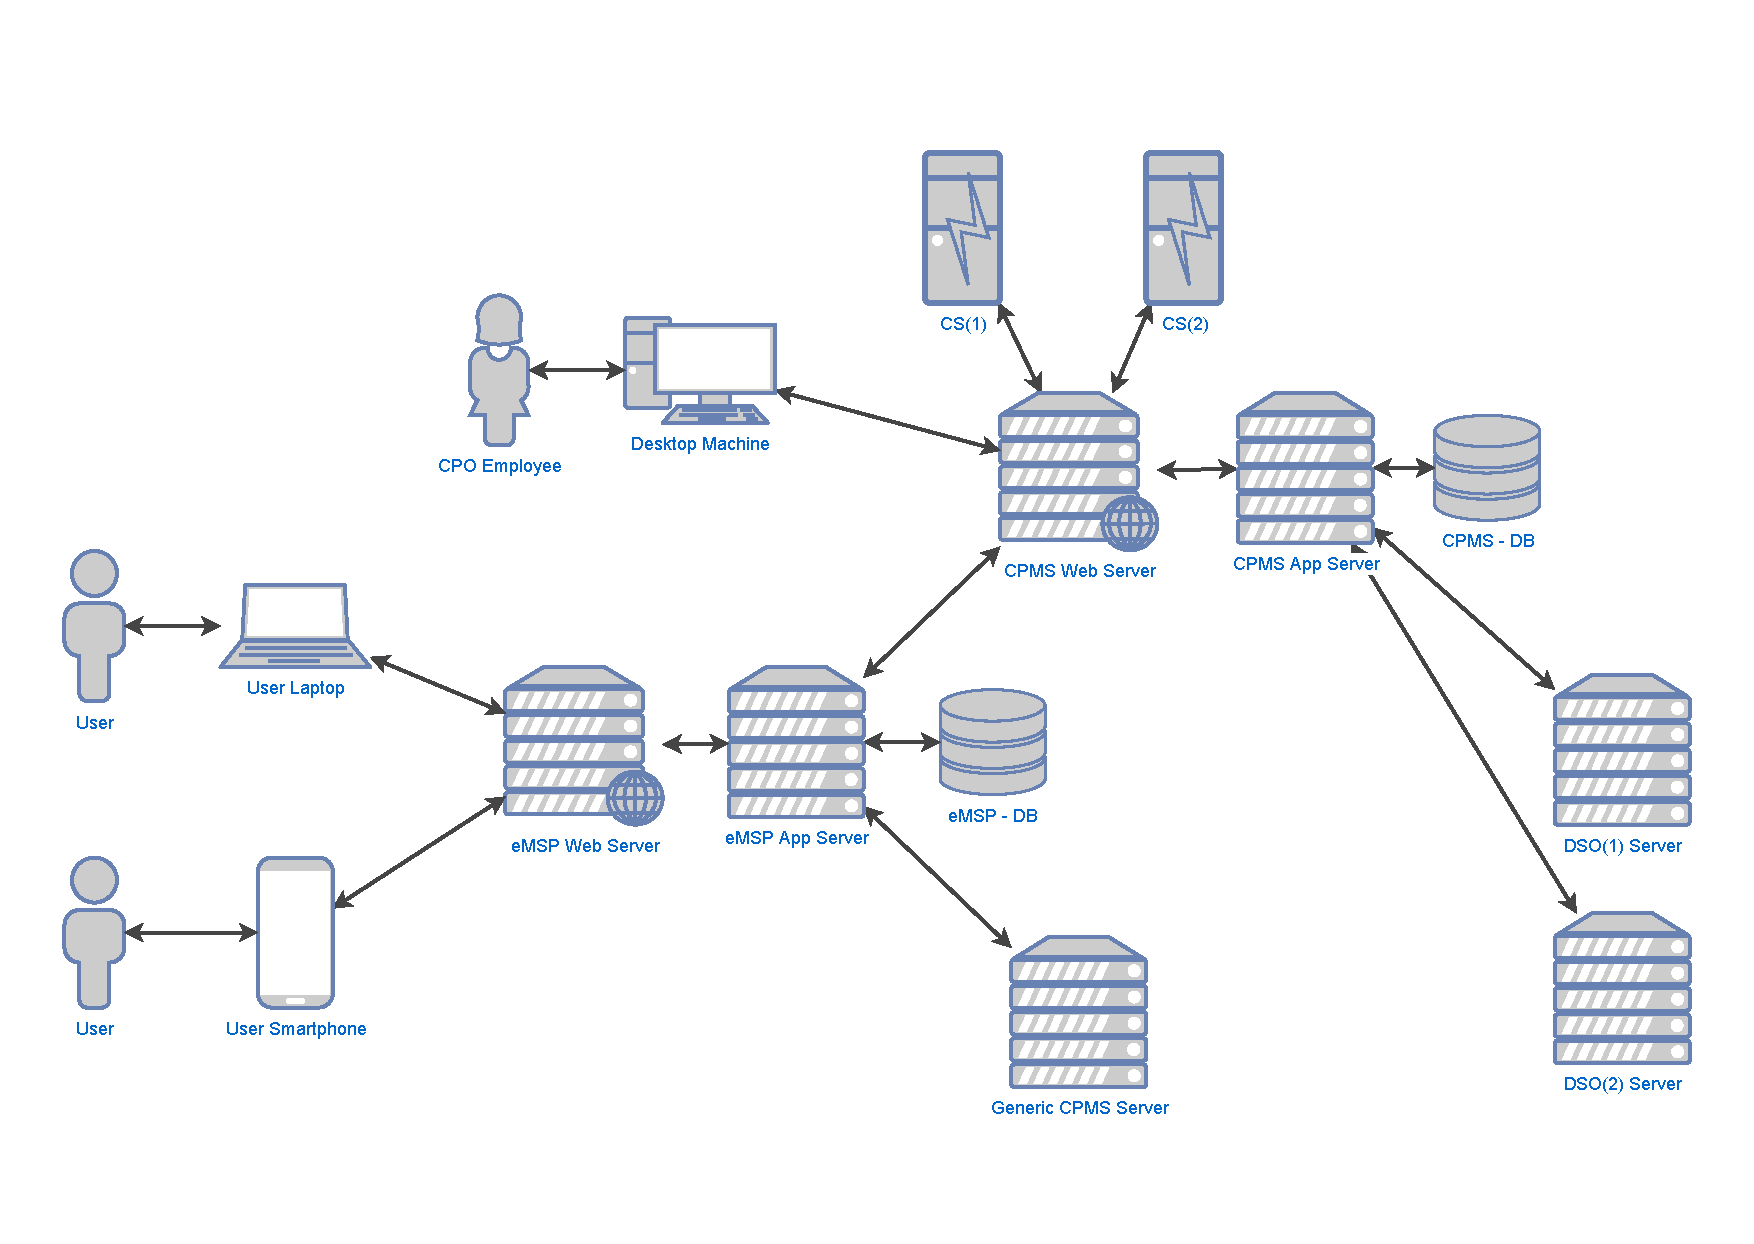
\includegraphics[page={1}, trim=1cm 1.25cm 1cm 1.25cm, width=\linewidth, clip]{OverviewDiagram.pdf}
    \caption{Overview Diagram}
\end{figure}

\begin{itemize}
    \item \textbf{eMSP Web Application} \\
        A Web Application that runs within the User’s web browser and that gives them access to the eMall services. All the resources it needs get downloaded to the User's browser from the eMSP Web Server as the the device reaches it through HTTP requests.

    \newpage

    \item \textbf{eMSP Web Server} \\
        Back-end component that interfaces the User's web browser with the other application services in the eMSP's back-end. It handles HTTP requests arriving from user-devices by routing them to the corresponding components that can respond to them.
    \item \textbf{eMSP App Server} \\
        The principal back-end component for the eMSP, it contains all the modules that together offer all functionalities available via the eMSP. Requests are routed from the Web Server to the module capable handling them, the response is than sent from the App Server through the Web Server to the User's device. The App Server is also capable of accessing the eMSP DB and the external services needed for its functions.
    \item \textbf{eMSP DB Server} \\
        Component dedicated to data storage for the eMSP, it stores for instance the Users' credentials and bookings, to ensure its safety it can only be accessed by the eMSP's App Server.
    \item \textbf{CPMS Web Application} \\
        A Web Application meant for the desktop devices available to CPO Employees, it runs withing the browser and allows its users to access the management functions of the CPMS. It dialogues with the CPMS Web Server through the HTTP protocol.
    \item \textbf{CPMS Web Server} \\
        Back-end component that interfaces the CPO Employees' web browser and the back-ends of the eMSP with the application services in the CPMS's back-end. It handles HTTP requests arriving from the outside by routing them to the corresponding components that can respond to them and allows tunneling of WebSocket connections from CS to the back-end.
    \item \textbf{CPMS App Server} \\
        The principal back-end component for the CPMS, it contains all the modules that together offer all functionalities available to the CPO and eMSPs, as well as being the endpoint where CS connect to in order to be managed. Requests and connections are routed from the Web Server to the module capable handling them, in the fist case the response is than sent from the App Server through the Web Server to the requesting device, in the second case the connection is handled and kept alive by its target module. The App Server is also capable of accessing the CPMS DB and the external services needed for its functions.
    \item \textbf{CPMS DB Server} \\
        Component dedicated to data storage for the CPMS, it stores for instance the credentials for CPO Employees as well as a local copy of the CSs' configurations, to ensure its safety it can only be accessed by the CPMS's App Server.
    \item \textbf{CS} \\
        External entity w.r.t. the STB, it is configured to reach out to the CPMS App Server via a WebSocket connection that allows the CPMS to manage and monitor it.
    \item \textbf{DSO} \\
        External entity w.r.t. the STB, it exposes a web API that allows CPMSs to acquire information regarding its price and energy mix.
    \item \textbf{Maps Provider} \\
        External entity w.r.t. the STB, offers to clients up to date maps of any requested area, as well as related information such as satellite images.
\end{itemize}

\subsection{Component View}

In this section, every major component is analysed in terms of its sub-components. \\
Everything that is outside of the system is considered as a black box.

\newpage

\begin{figure}[!ht]
    %trim = left bottom right top
    \centerline{
        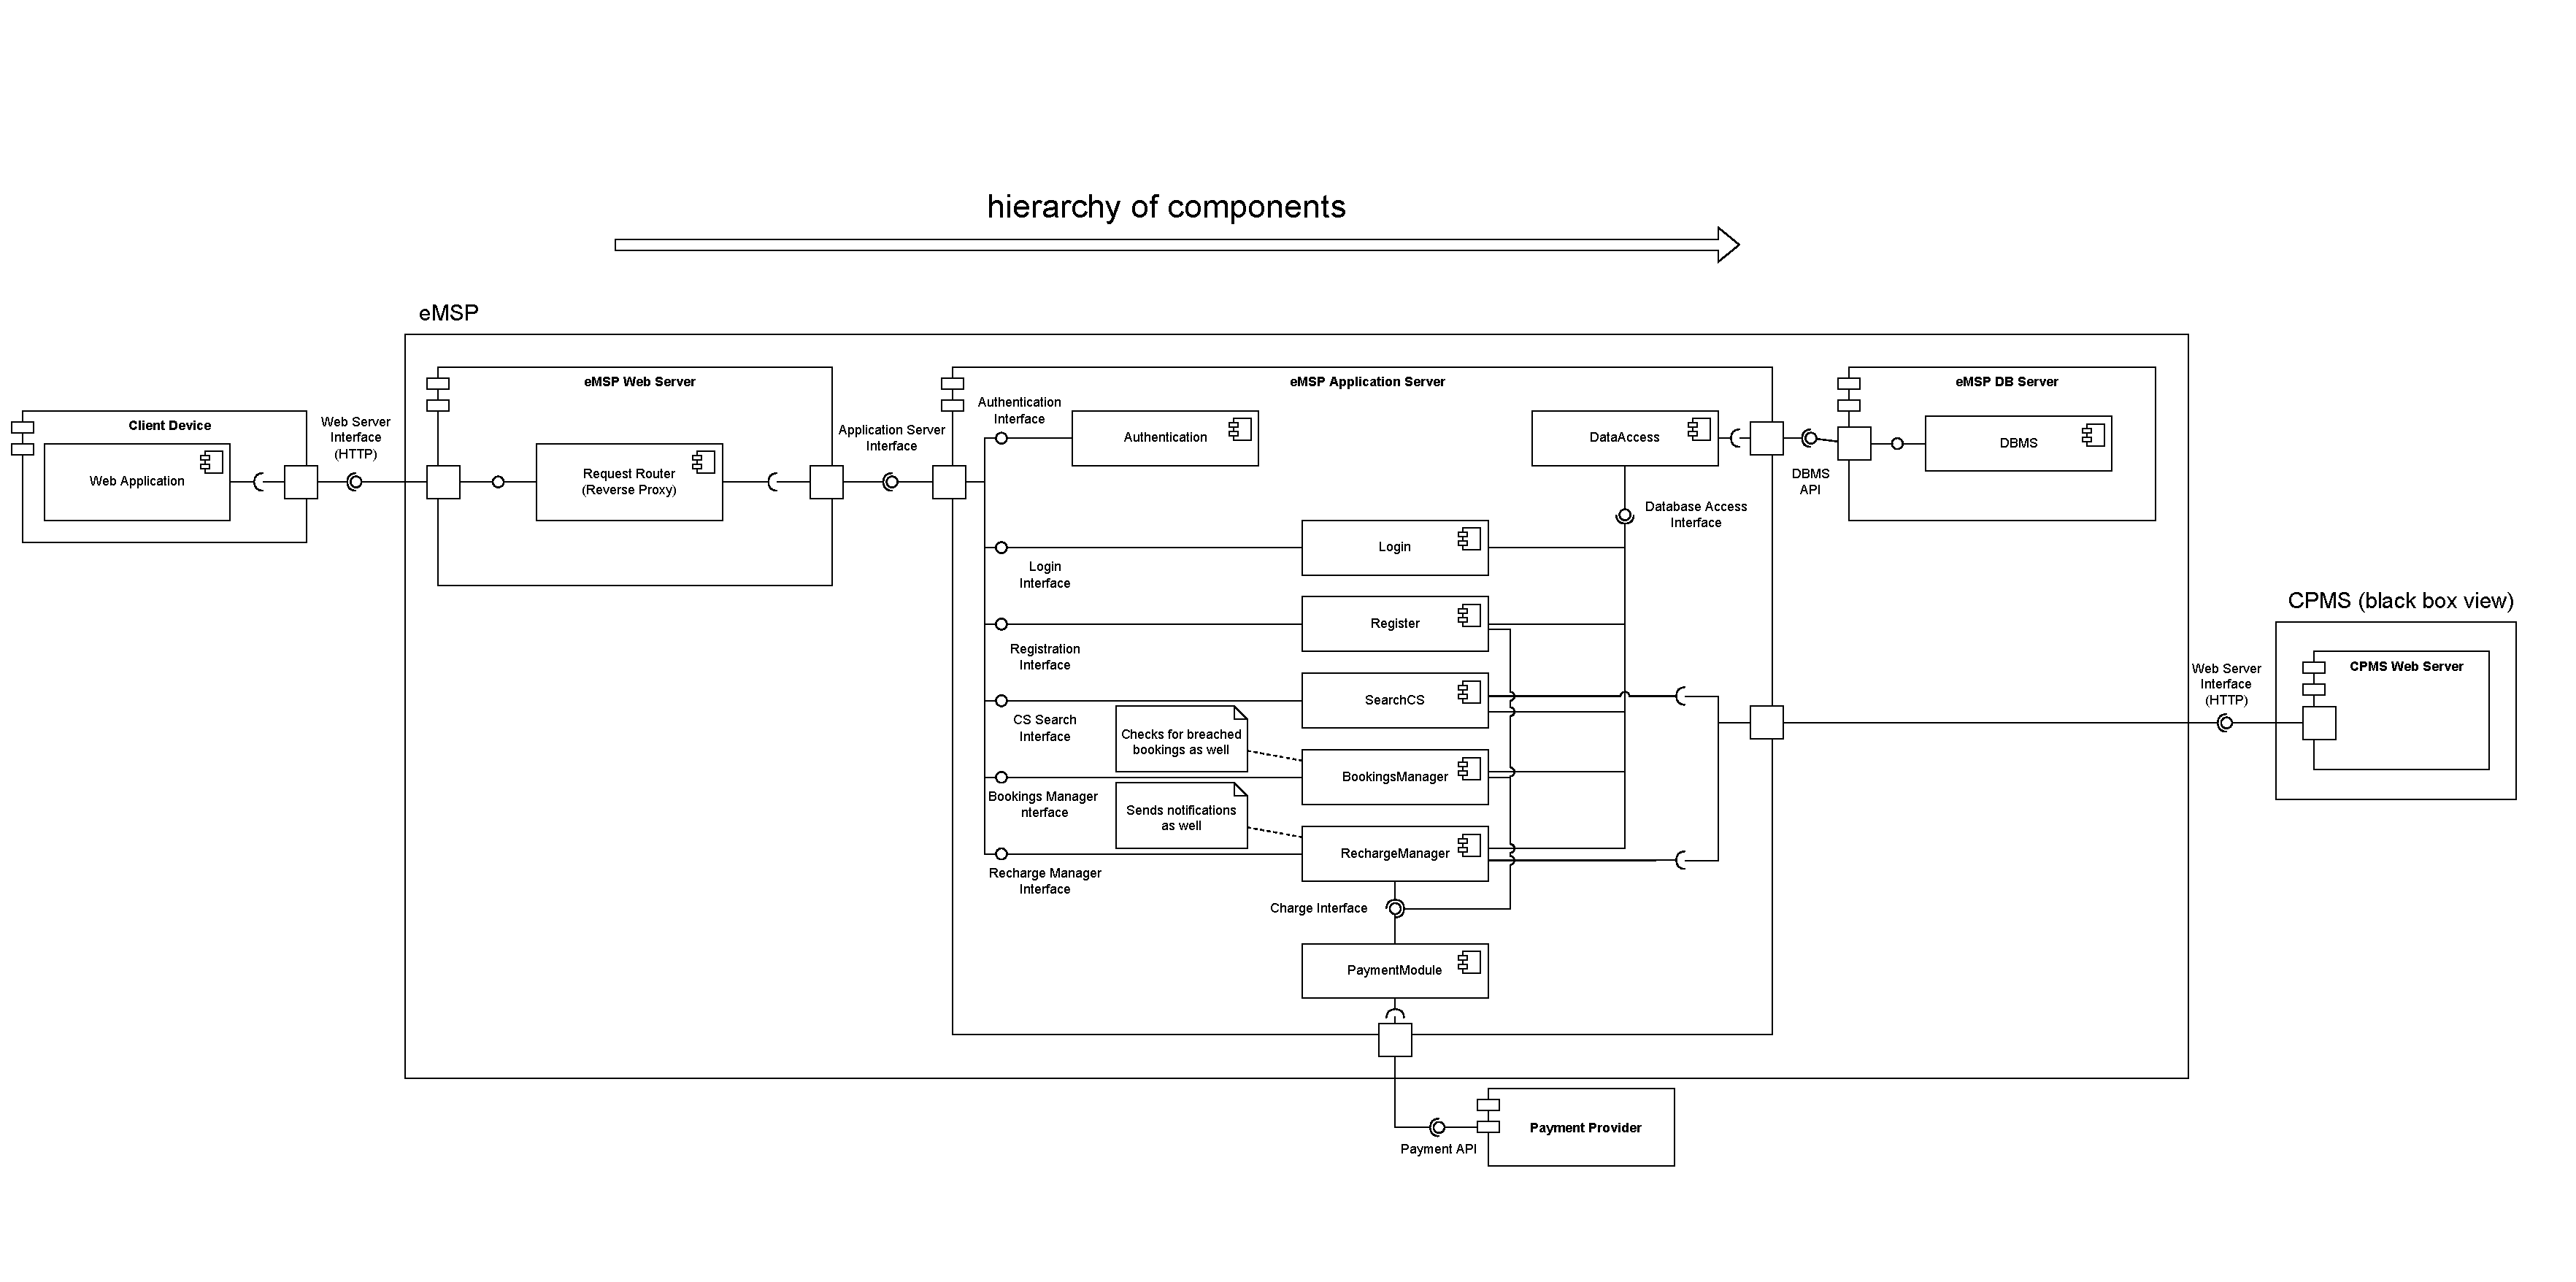
\includegraphics[page={1}, width=1.26\linewidth, trim=0cm 2cm 0cm 4cm, angle=-90, clip]{ComponentDiagram.pdf}
    }
    \caption{Component diagram}
\end{figure}

\newpage

\begin{figure}[!ht]
    %trim = left bottom right top
    \centerline{
        \includegraphics[page={2}, width=1.26\linewidth, trim=3cm 1cm 4cm 3cm, angle=-90, clip]{ComponentDiagram.pdf}
    }
    \caption{Component diagram}
\end{figure}

\newpage

\subsubsection{Client Device}

Client devices represent all the devices connected to the internet and used to reach the eMall website. By reaching eMall the \textbf{eMSP Web Application Component} in the form of an interactive web application is loaded by the device's web browser and eMall's UI is shown to the User.\\
\\
The \textbf{eMSP Web Application Component} is the front-end that it offers to its Users, it consists of a website offering an interactive web application with a UI that allows Users to access every function offered by eMall. This component does not integrate computational intensive tasks and in itself does not have any data that can instead be provided by eMall's back-end. Its functionalities are limited to error checking, UI rendering and contacting the eMSP's back-end to recover any data needed to offer the User the intended functionalities.

\subsubsection{eMSP Web Server Component}

The eMSP Web Server is required in order to serve the eMSP Web Application to User, and to allow such Web App to interact with the eMSP's back-end when needed. \\
\\
To this end its main sub-component is a \textbf{Request Router}, a Reverse Proxy component that sits in front of the back-end and routes requests from client devices to the back-end services capable of satisfying them, this way the resources returned to clients appear as if they originated from the Web Server itself. \\
The role of the Reverse Proxy is also to help increase scalability, performance, resilience and security by both acting as a content cache and as a middleware before the back-end. 

\subsubsection{eMSP Application Server Component}

The back-end for the eMSP, as per the hierarchy of components, every request reaching it is first checked for an active session, and only those with one which has a performed valid login are allowed access to components other than \textbf{Register}. \\
Every component present performs all the required checks on the received data to correctly perform any of its functions.

\begin{itemize}
    \item \textbf{Authentication} \\
        Sub-component that handles the authentication by checking the credentials for every request reaching the back-end.
    \item \textbf{Login} \\
        Sub-component which checks the login credentials inserted by Users through the Web App and grants them an authenticated session if those are valid.
    \item \textbf{Register} \\
        Sub-component that allows Unregistered Users to create a new account with eMall.
    \item \textbf{SearchCS} \\
        Sub-component whose purpose is to allow authenticated Users to query eMall for the CSs it has available with the use of filters. It returns the list of matching CSs.
    \item \textbf{BookingsManager} \\
        Sub-component offering the functionalities to both create a new booking and receive the current list of bookings for the authenticated User, with the possibility of deleting any booking. 
    \item \textbf{RechargeManager} \\
        Sub-component which allows for control over a booking which is currently active, after a User has connected their vehicle to a booked CS, via this component they can start/stop the charging process as well as get notified of the process terminating.
    \item \textbf{PaymentModule} \\
        Sub-component that interfaces with an external payment provider and allows the eMSP to charge Users for any obtained service or fee if they were not to show up for a booking.
    \item \textbf{DataAccess} \\
        Sub-component that provides access to the DB for every other sub-component.
\end{itemize}

\subsubsection{CPO Device}

CPO Devices represent all the machines available to CPO Employees to operate with the company's CPMS. \\
\\
The \textbf{CPMS Web Application Component} is meant to be ran inside a web browser on the CPO Devices and consequently be available to CPO Employees, it is the front-end offered by the CPMS and its UI is meant to offer to its users all the management functionalities of the CPMS. This component does not integrate computational intensive tasks and does not store locally any data that can instead be provided by the CPMS's back-end. Its functionalities are limited to error checking, UI rendering and contacting the CPMS's back-end to recover any data required for its functionalities.

\subsubsection{CPMS Web Server Component}

The CPMS Web Server is required in order to serve the CPMS Web Application to CPO Employees, to allow such Web App to interact with the CPMS's back-end and to allow CS to reach the CPMS with a WebSocket connection, allowing the CPMS to actively manage them. \\
\\
To this end its main sub-components are:

\begin{itemize}
    \item \textbf{Request Router} \\
        A reverse proxy that sits between a client and the CPMS back-end, its role is to route requests from clients to the back-end services capable of answering them, this way the resources resources returned to clients appear as if they originated from the Web Server itself. The role of the Reverse Proxy is also to help increase scalability, performance, resilience and security by both acting as a content cache and as a middleware before the back-end.
    \item \textbf{WebSocket Proxy} \\
        Its role is to tunnel WebSocket connections between the CPMS back-end and the CSs, after those are originated from upgrade requests over HTTP that went through the Request Router.
\end{itemize}

\subsubsection{CPMS Application Server Component}

The back-end for the CPMS, every request reaching it is let through to the CPO-only components only if it has an active authenticated session with CPO credentials. Access to components that are meant for eMSPs is granted to all eMSPs that are known by the system as long as their request are correctly performed with an authenticated session. \\
Every component present performs all the required checks on the received data to correctly perform any of its functions.

\begin{itemize}
    \item \textbf{Authentication} \\
        Sub-component that handles the authentication by checking the credentials for every request reaching the back-end.
    \item \textbf{Login} \\
        Sub-component which checks the login credentials inserted by CPO Employees through the Web App and grants them an authenticated session if those are valid.
    \item \textbf{CSBatteryPolicyManager} \\
        Sub-component that allows CPOs to change the policy currently in use by a CS to manage its batteries, it both saves to the CPMS's DB updated CS policies as well as requests the \textbd{CSManager} to communicate the updated policies to the actual CS.
    \item \textbf{CSDSOManager} \\
        Sub-component that allows CPOs to change the DSO currently supplying a CS, it both saves to the CPMS's DB updated CS's DSO as well as requests the \textbd{CSManager} to communicate the change to the actual CS.
    \item \textbf{CSPricesManager} \\
        Sub-component that allows CPOs to change the user-price, the nominal-price and the offer reset date of a CS, it both saves to the CPMS's DB updated prices and date as well as requests the \textbd{CSManager} to communicate the updated values to the actual CS.
    \item \textbf{AutomaticModeManager} \\
        Sub-component which allows CPO Employees to toggle the operating mode of the CPMS from “Automatic Mode” to “Manual Mode” or vice-versa, as well as allowing the CPO to update the CPMS’s policy for “Automatic Mode”.
    \item \textbf{CSList} \\
        Sub-component providing the CPO and external eMSPs with the list of CS currently under the control of the CPMS. It also accepts filters to reduce the list of provided CSs. If they are requested, details regarding a specific CS can also be provided by this component.
    \item \textbf{RechargeManager} \\
        Sub-component providing external eMSPs with the possibility of managing, on behalf of their Users, the ongoing charging process to a certain socket of a CS. This module also provides the eMSP feedback on the current status of the charging process. This component dialogues with the \textbd{CSManager} to gather the CS status and forward it commands to manage the charging process.  
    \item \textbf{DSOInformation} \\
        Sub-component providing the CPO with information regarding the DSOs known by the CPMS. This module also interfaces directly with the DSOs external API to gather their prices and energy mixes. 
    \item \textbf{CSManager} \\
        Sub-component that allows the other back-end components to dialogue with CSs, know their real-time status, coordinate their charging processes and update their configuration. CS signal this module when one of their recharges is complete, and this module forwards such notification to the eMSP. This module also accepts WebSocket connections from CS to allow their management.
    \item \textbf{DataAccess} \\
        Sub-component that provides access to the DB for every other sub-component.
\end{itemize}

\newpage

\subsubsection{eMSP DB Components}

SQL DB for the eMSP, it contains the accounts and bookings of all users.

%trim = left bottom right top
\begin{figure}[!ht]
    \centering
    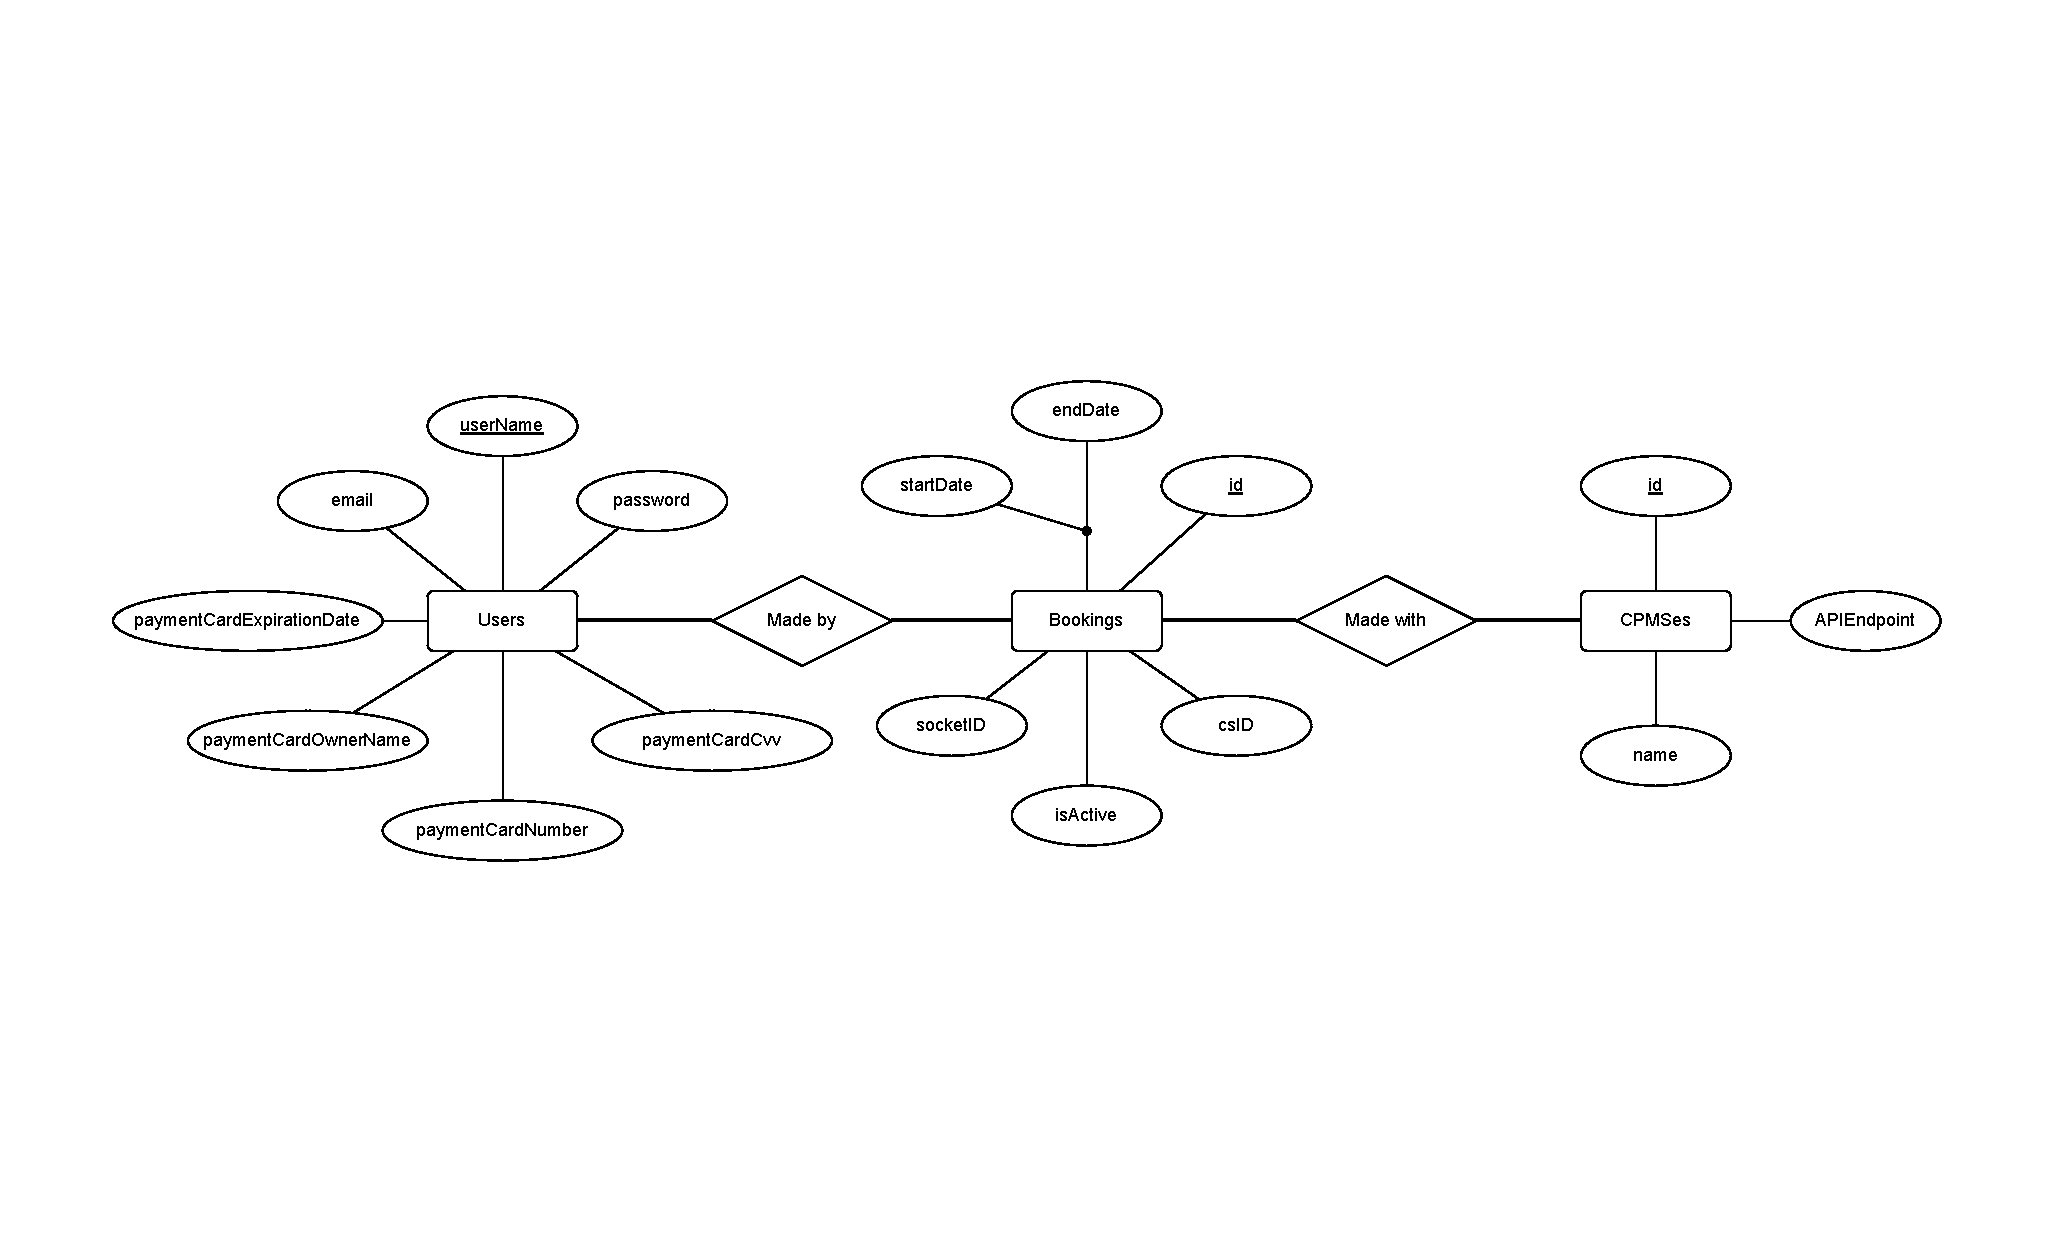
\includegraphics[page={1}, trim=1.5cm 6cm 1.5cm 6cm, width=\linewidth, clip]{ERDiagrams.pdf}
    \caption{eMSP ER Diagram}
\end{figure}

\subsubsection{CPMS DB Components}

SQL DB for the CPMS, it contains information on all known CSs and their configurations.

%trim = left bottom right top
\begin{figure}[!ht]
    \centering
    \includegraphics[page={2}, trim=5cm 3.5cm 5cm 3.5cm, width=\linewidth, clip]{ERDiagrams.pdf}
    \caption{CPMS ER Diagram}
\end{figure}

\newpage

\subsubsection{External Systems}

Systems outside the scope of this document, whose existence is acknowledge in order to explain the behaviour of certain components of the STB.

\begin{itemize}
    \item \textbf{DSO} \\
        An endpoint with an exposed API that allows for retrieval of information regarding the DSO's energy mix and prices.
    \item \textbf{Payment Provider} \\
        An endpoint that allows, given adequate payment details, to charge someone for a service and move the sum to a certified bank account.
    \item \textbf{Map Provider} \\
        A service providing up to date maps for the entire world. It is reached by the eMSP Web Application to improve the UI with an interactive map.
\end{itemize}

\newpage

\subsection{Deployment View}

Here we describe the arrangement of physical nodes and the components deployed on them. \textbf{Load balancers} and \textbf{Firewalls} are also included in the diagram:
\begin{itemize}
    \item \textbf{Firewall} \\
        Is directly connected to the Internet and filters incoming packets, only letting pass those identified as trustworthy.
    \item \textbf{Load balancer} \\
        A device that forwards requests to the back-end's services in accordance to their current load, aiming to distribute work evenly. Its presence improves the maximum load capacity the system can handle and its reliability. 
\end{itemize}

%trim = left bottom right top
\begin{figure}[!ht]
    \centering
    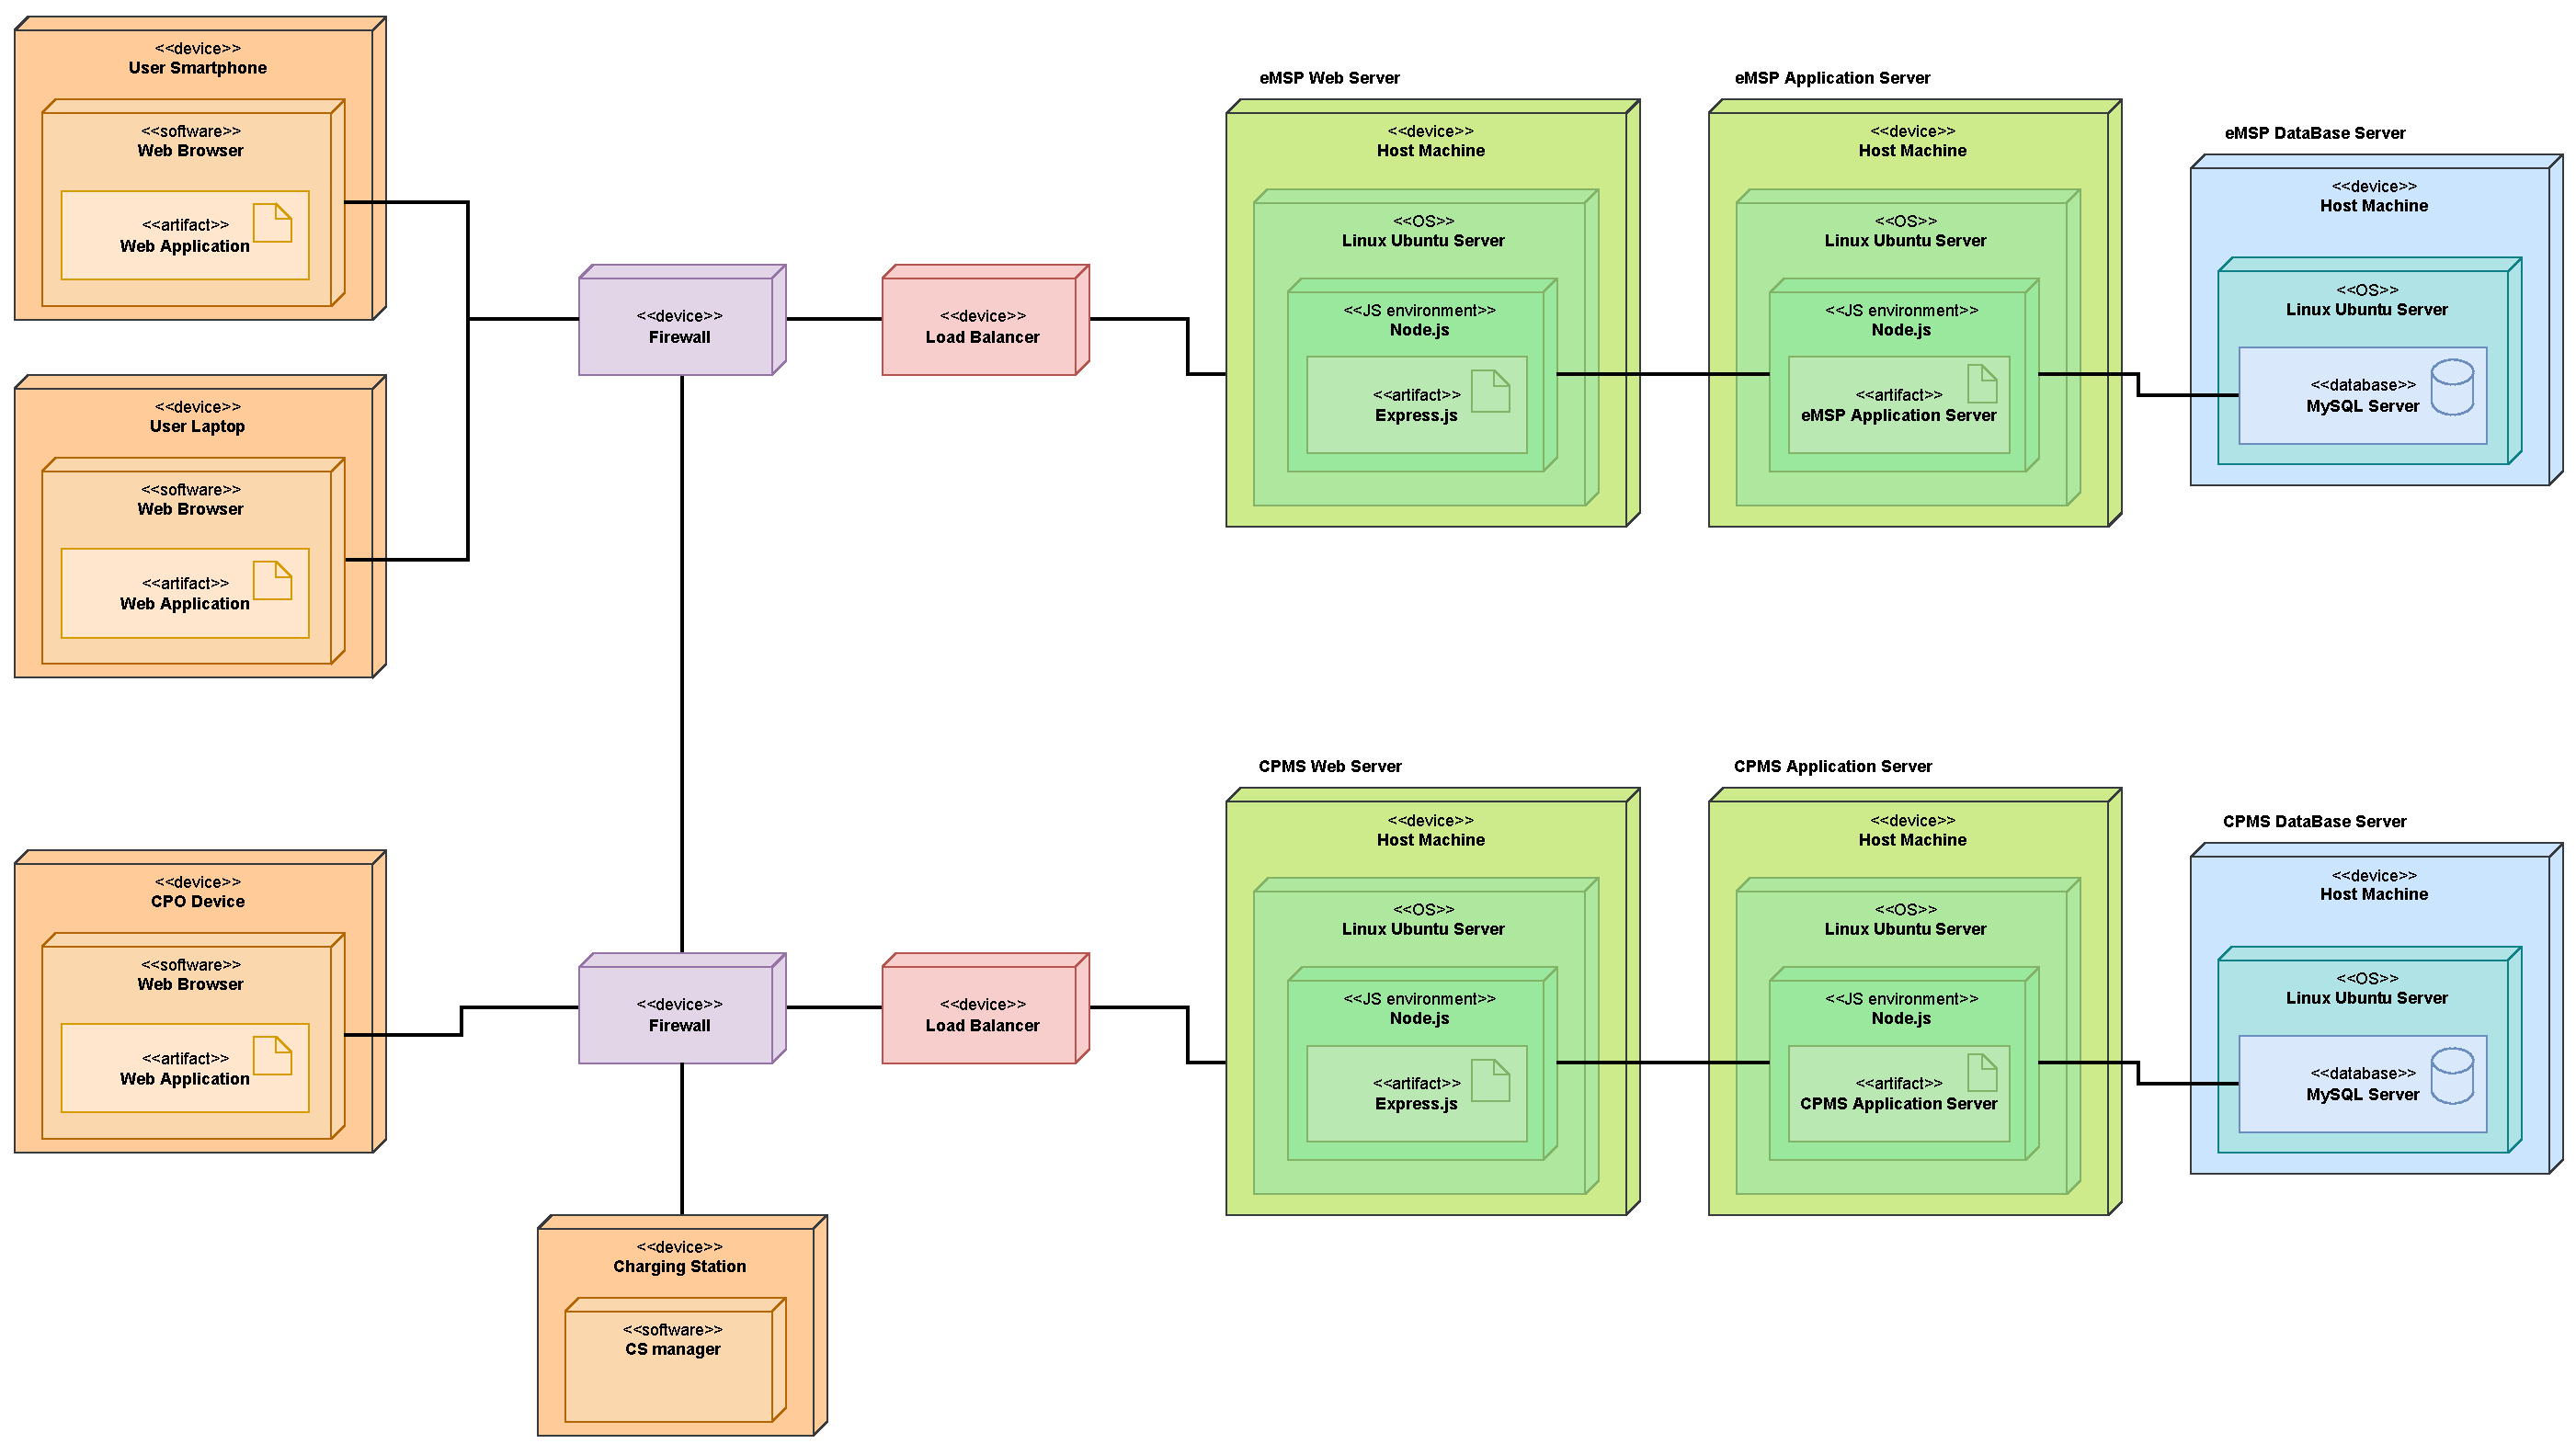
\includegraphics[page={1}, trim=0cm 0cm 0cm 0cm, width=\linewidth, clip]{DeploymentView.pdf}
    \caption{Deployment View}
\end{figure}
    
Client devices will only need to reach the Web Server of the eMSP, which will then forward their requests to the eMSP's back-end if needed.

\newpage

\subsection{Runtime View}

In this section the dynamic behaviour of the system is presented via sequence diagrams that summarize all the possible interactions that can be had with both the eMSP or the CPMS. Each diagram further expands on those discussed in the RASD document in section 3.2.3 .

\begin{description}
    \item \textbf{1. New user registration}
    %trim = left bottom right top
    \begin{figure}[!ht]
        \centering
        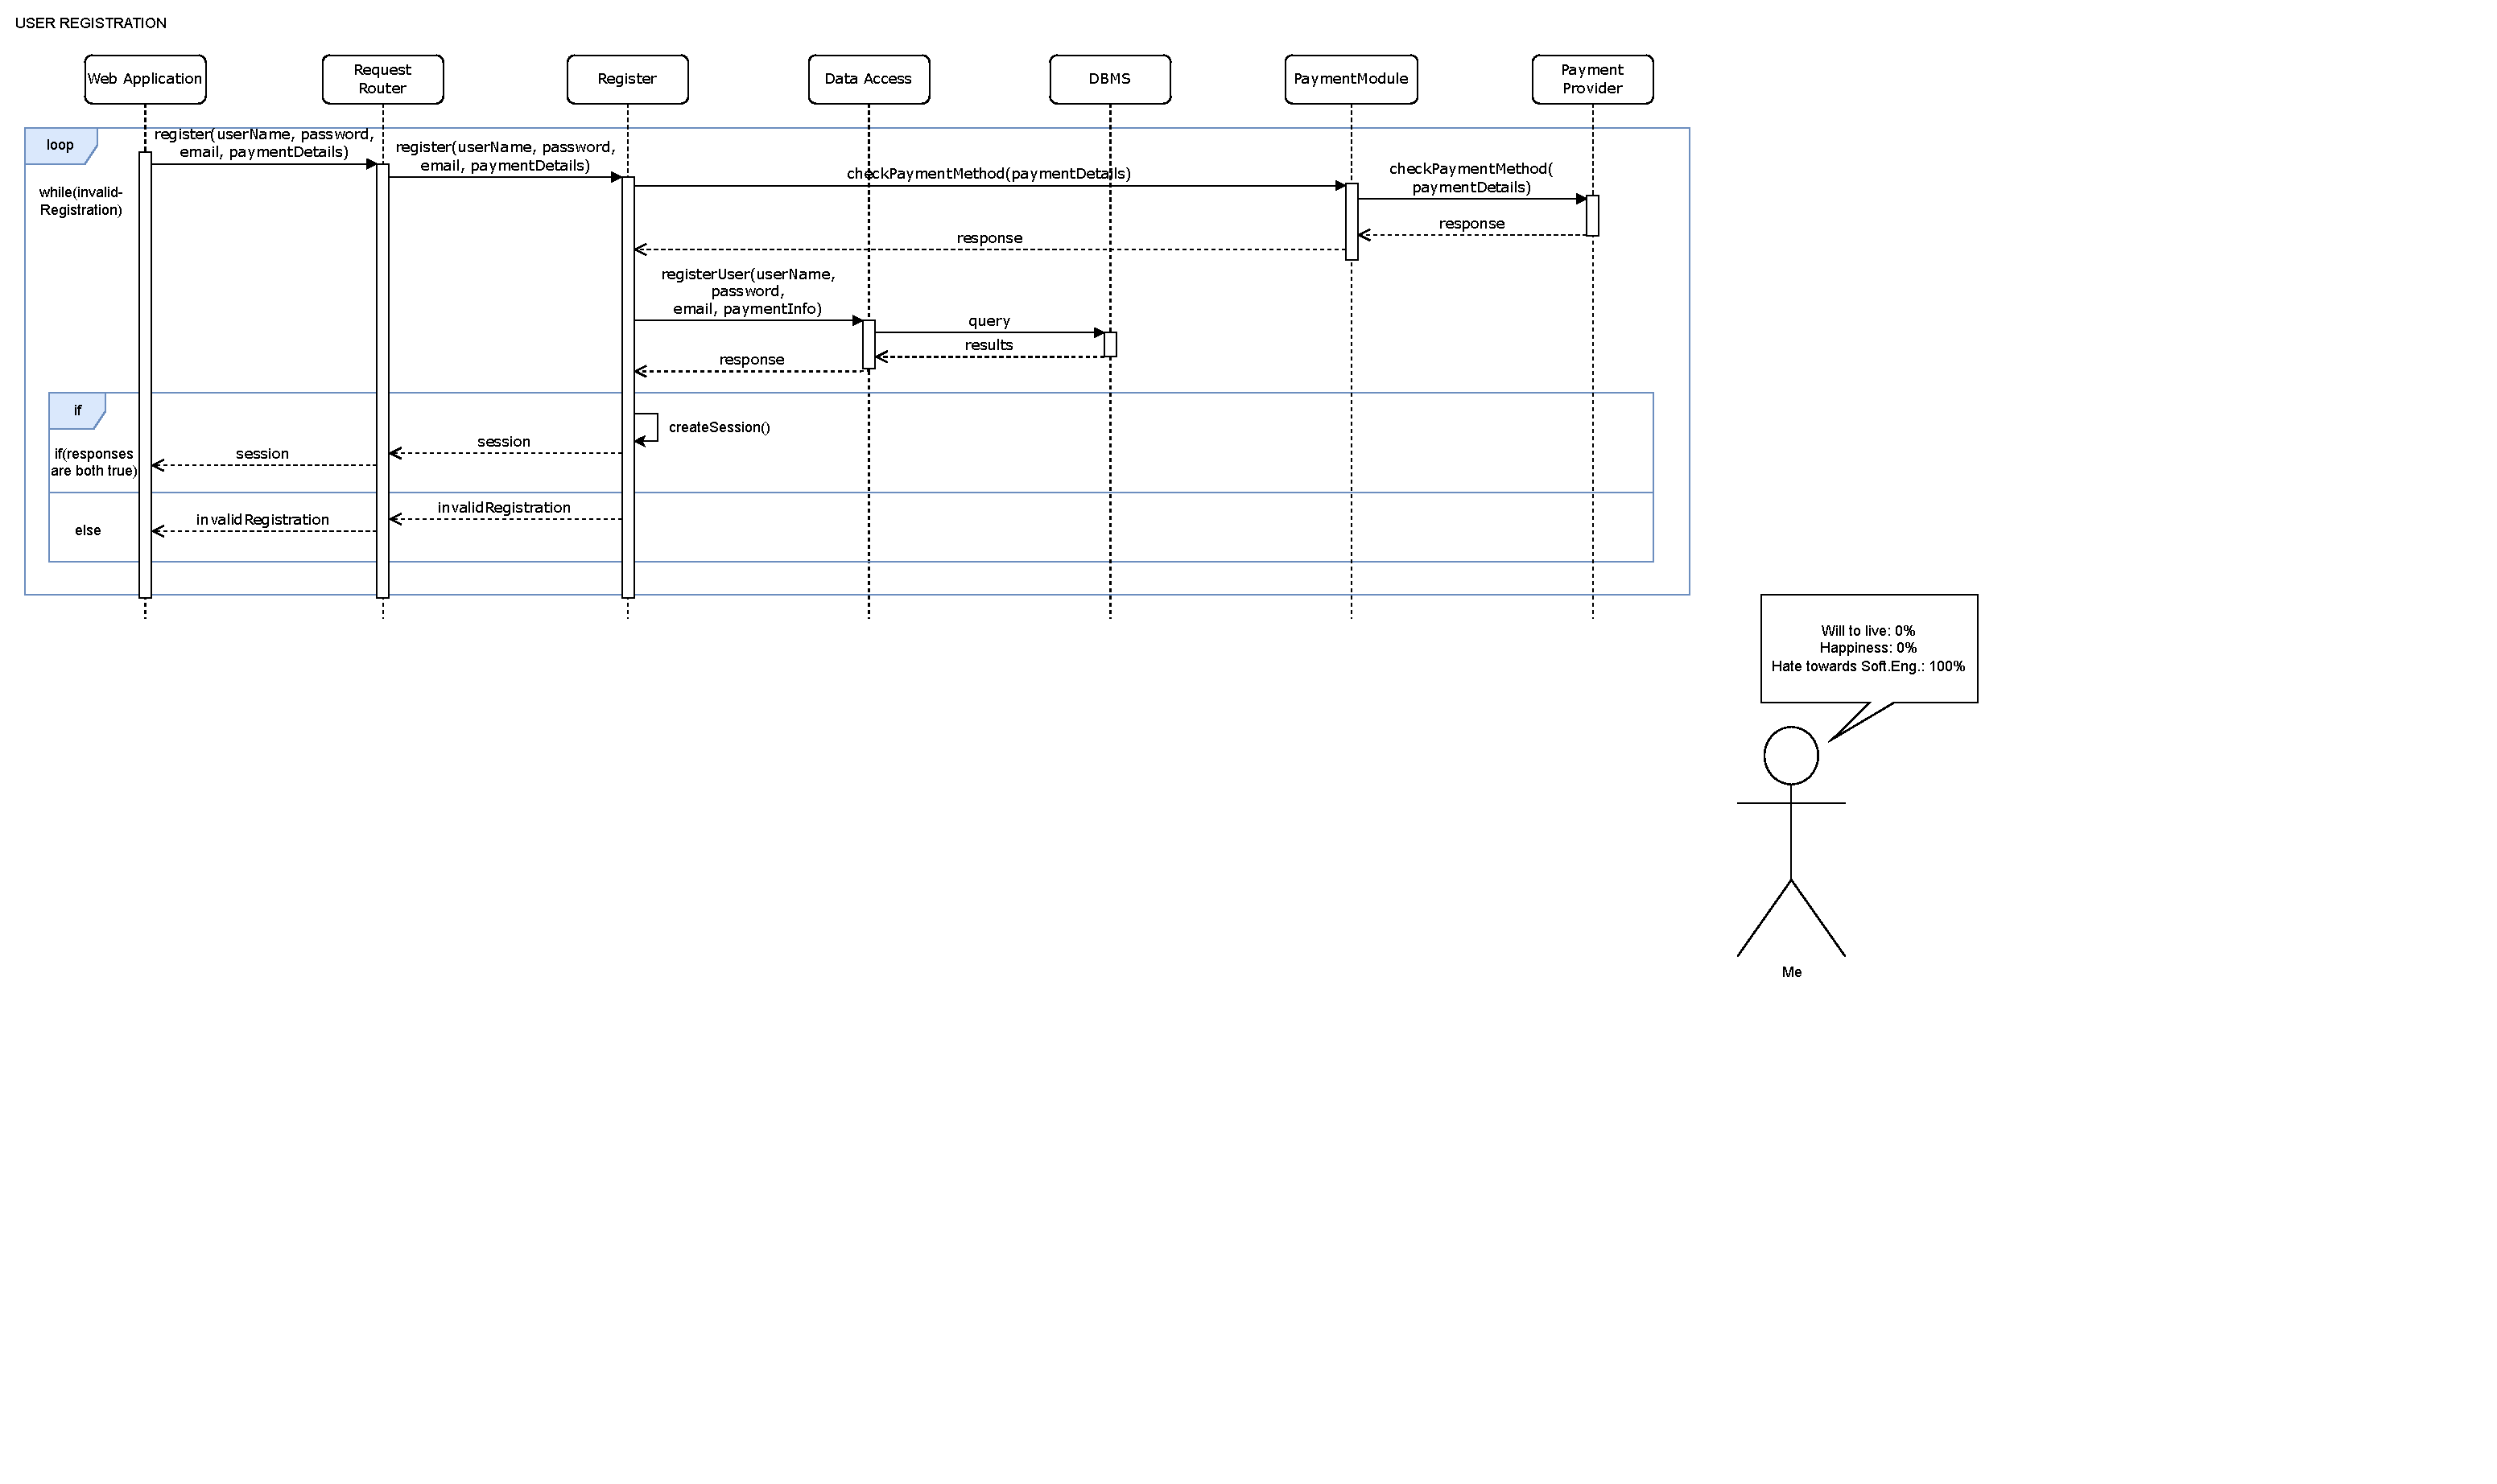
\includegraphics[page={1}, trim=0cm 18cm 16cm 1cm, width=\linewidth, clip]{RuntimeDiagrams.pdf}
        \caption{New user registration}
    \end{figure}
    
    \item \textbf{2. User login}
    %trim = left bottom right top
    \begin{figure}[!ht]
        \centering
        \includegraphics[page={2}, trim=0cm 20cm 25cm 1cmm, width=\linewidth, clip]{RuntimeDiagrams.pdf}
        \caption{User login}
    \end{figure}
    
    \newpage
    
    \item \textbf{3. User searching and booking a CS}
    %trim = left bottom right top
    \begin{figure}[!ht]
        \centering
        \includegraphics[page={3}, trim=0cm 5cm 0cm 1cmm, width=\linewidth, clip]{RuntimeDiagrams.pdf}
        \caption{User login}
    \end{figure}
    
    \item \textbf{4. User deleting one of his bookings}
    %trim = left bottom right top
    \begin{figure}[!ht]
        \centering
        \includegraphics[page={4}, trim=0cm 10cm 21cm 1cmm, width=0.95\linewidth, clip]{RuntimeDiagrams.pdf}
        \caption{User deleting one of his bookings}
    \end{figure}
    
    \newpage
    
    \item \textbf{5. User starting a charging process}
    %trim = left bottom right top
    \begin{figure}[!ht]
        \centering
        \includegraphics[page={5}, trim=0cm 7cm 8cm 1cmm, width=\linewidth, clip]{RuntimeDiagrams.pdf}
        \caption{User starting a charging process}
    \end{figure}
    
    \item \textbf{6. User interrupting a charging process}
    %trim = left bottom right top
    \begin{figure}[!ht]
        \centering
        \includegraphics[page={6}, trim=0cm 3cm 1cm 1cmm, width=\linewidth, clip]{RuntimeDiagrams.pdf}
        \caption{User interrupting a charging process}
    \end{figure}
    
    \newpage
    
    \item \textbf{7. Charging procedure self-terminates and User receives a notification}
    %trim = left bottom right top
    \begin{figure}[!ht]
        \centering
        \includegraphics[page={7}, trim=0cm 16cm 0cm 1cmm, width=\linewidth, clip]{RuntimeDiagrams.pdf}
        \caption{Charging procedure self-terminates and User receives a notification}
    \end{figure}
    
    \item \textbf{8. User does not show up for a booked recharge}
    %trim = left bottom right top
    \begin{figure}[!ht]
        \centering
        \includegraphics[page={8}, trim=0cm 19cm 26cm 1cmm, width=0.8\linewidth, clip]{RuntimeDiagrams.pdf}
        \caption{User does not show up for a booked recharge}
    \end{figure}
    
    \item \textbf{9. CPO logs in into the CPMS}
    %trim = left bottom right top
    \begin{figure}[!ht]
        \centering
        \includegraphics[page={9}, trim=0cm 20cm 25cm 1cmm, width=0.95\linewidth, clip]{RuntimeDiagrams.pdf}
        \caption{CPO logs in into the CPMS}
    \end{figure}
    
    \newpage
    
    \item \textbf{10. CPO retrieves energy prices and mixes from DSOs}
    %trim = left bottom right top
    \begin{figure}[!ht]
        \centering
        \includegraphics[page={10}, trim=0cm 17cm 25cm 1cmm, width=\linewidth, clip]{RuntimeDiagrams.pdf}
        \caption{CPO retrieves energy prices and mixes from DSOs}
    \end{figure}
    
    \newpage
    
    \item \textbf{11. CPO assigns nominal-price, user-price, energy sources and battery usage policies for a CS} \\
    %trim = left bottom right top
    \begin{figure}[!ht]
        \centering
        \includegraphics[page={11}, trim=0cm 4cm 1cm 1cm, width=\linewidth, clip]{RuntimeDiagrams.pdf}
        \caption{CPO assigns nominal-price, user-price, energy sources and battery usage policies for a CS}
    \end{figure} \\
    This diagram summarized 3 views in one, by simply substituting the following components and interactions to the $\ast s$ one can obtain the different versions:
    \begin{enumerate}
        \item \textbf{CPO assigns nominal-price, user-price}
        \begin{description}
            \item $\ast\ \rightarrow$ CSPricesManager
            \item $\ast\ast \rightarrow$ updateCSPrices(CSID, userprice, nominalprice)
            \item $\ast\ast\ast \rightarrow$ updateCSPrices(userprice, nominalprice)
        \end{description}
        \item \textbf{CPO assigns energy sources}
        \begin{description}
            \item $\ast \rightarrow$ CSDSOManager
            \item $\ast\ast \rightarrow$ updateCSDSO(CSID, DSOId)
            \item $\ast\ast\ast \rightarrow$ updateCSDSO(DSOId)
        \end{description}
        \item \textbf{CPO assigns energy battery usage policies}
        \begin{description}
            \item $\ast \rightarrow$ CSBatteryPolicyManager
            \item $\ast\ast \rightarrow$ updateCSBatteryPolicy(CSID, thresholds, weights)
            \item $\ast\ast\ast \rightarrow$ updateCSBatteryPolicy(thresholds, weights)
        \end{description}
    \end{enumerate}
    
    \newpage
    
    \item \textbf{12. CPO toggles the CPMS operating mode}
    %trim = left bottom right top
    \begin{figure}[!ht]
        \centering
        \includegraphics[page={12}, trim=0cm 16cm 28cm 1cmm, width=0.95\linewidth, clip]{RuntimeDiagrams.pdf}
        \caption{CPO toggles the CPMS operating mode}
    \end{figure}
    
    \item \textbf{13. CPO changes the CPMS’s “Automatic Mode” policy}
    %trim = left bottom right top
    \begin{figure}[!ht]
        \centering
        \includegraphics[page={13}, trim=0cm 15cm 27cm 1cmm, width=0.95\linewidth, clip]{RuntimeDiagrams.pdf}
        \caption{CPO changes the CPMS’s “Automatic Mode” policy}
    \end{figure}
\end{description}
%Salve!
%Ciao! Come va?
%Ho un pelo di febbre...però a parte quello tutto bene dai!
%Ahio... iniziamo l'anno?
%Ma neh ahahah, pace, tanto sicuramente ho preso freddo, un giono al massimo e sto bene! Tu invece, tutto ok?
%Eh col tempo che c'è tra l'altro... Ma sei qui a Milano?
%Nono, a casetta al calduccio ahaha, a Milano non ci metto piede almeno fino all'esame di FOR
%E fai bene ahaha qui è grigio e piove tutti i giorni :sad:
%BTW stavo pensando: per descrivere l'architettura non ci conviene splittare (almeno nella overview dove spieghiamo un po' tutto a grandi linee) la roba lato eMSP e CPMS?
%Mhhh, direi che si può fare tranquillamente, non so esattamente cosa scriveresti nelle due sezioni, ma se hai qualcosa in mente, vai pure!
%Onsetamente lato CPMS non so manco io cosa mettere, mi sembra tutto self-evident dal diagramma (che poi è venuto molto bene) però vabbè mi invento qualcosa sicuro!
%Onesto, allora al massimo inserisci la sezione extra solo per l'eMSP e pace...
%Aspe quale sezione extra?
%Se volevi aggiungere una descrizione "descrivere l'architettura non ci conviene splittare"
%Ah no io intendevo che nella overview spiego prima quella dell'eMSP (come sistema a sè) e poi quella del CPMS (come sistema a sè) quindi con tutte le tier ecc
%Ahhhh, sorry, avevo capito male, allora niente, va benissimo anche se scrivi un tot per l'eMSP e poi per il CPMS la chiudi in fretta perchè in effetti c'è ben poco da dire...
%Eh già, non c'è molto da dire per quello... Ok
%Perfetto, allora mentre tu fai quella parte io fixo due o tre cose che non mi piacciono dei diagrammi vari e poi ci sono da fare solo quelli dell'integration...
%Ovvero? Oh no l'integration.... Ma cosa non ti piace?
%Ah, solo qualche freccia non centrata o blocchi non allineati XD
%Aaah no pensavo che ci fosse roba strutturale da cambiare
%Nonono, spero quello di non doverci più mettere mano, anche perchè oramai il tempo non lo permette...
%Well... tecnicamente possiamo fare modifiche fino al 17 febbraio eh... però abbiamo anche gli esami e l'implementazione da fare, quindi non so quanto modificheremo
%No, infatti, io direi di finire coll'8-9 massimo e chiuderla lì col DD, fare l'implementazione ed al massimo tornare a fixare il DD a fine progetto, che tanto dalla mail dell'altro giorno ci è concesso!
%Concordo pienamente!
%Perfetto, allora io direi che stasera mi fixo i grafici e poi vado a dormire sperando di star meglio domani...poi che ne diresti domani sera o dopodomani di sentirci su discord per finire tutto?
%Se non ho call di DSD si può fare sì... magari dopo cena così sono un po' più sicuro di non avere nulla se ti va bene, altrimenti quando vuoi
%Assolutamente, tanto anche io fino alle 19 studio, quindi ci sarei alle ~21
%Ehehe idem
%Oki dai, allora ci sentiamo domani, se succede qualcosa con DSD fammi sapere any time!
%Sure!
%BTW abbiamo fatto un video di demo di DSD io ed Ema all'1 di notte... se vuoi ti mando il link
%Oddio ahahahahah, sono seriamente curioso XD
%Te lo mando su TG!
%Okkkk, nel mentre metto overleaf in background, 'Notte!
%Notte!

\newpage

\subsection{Component Interfaces}

This section provides a summary of the interfaces required and offered by the various components of both the eMSP and CPMS in the form of the following diagram.

\begin{figure}[!ht]
    %trim = left bottom right top
    \centerline{
        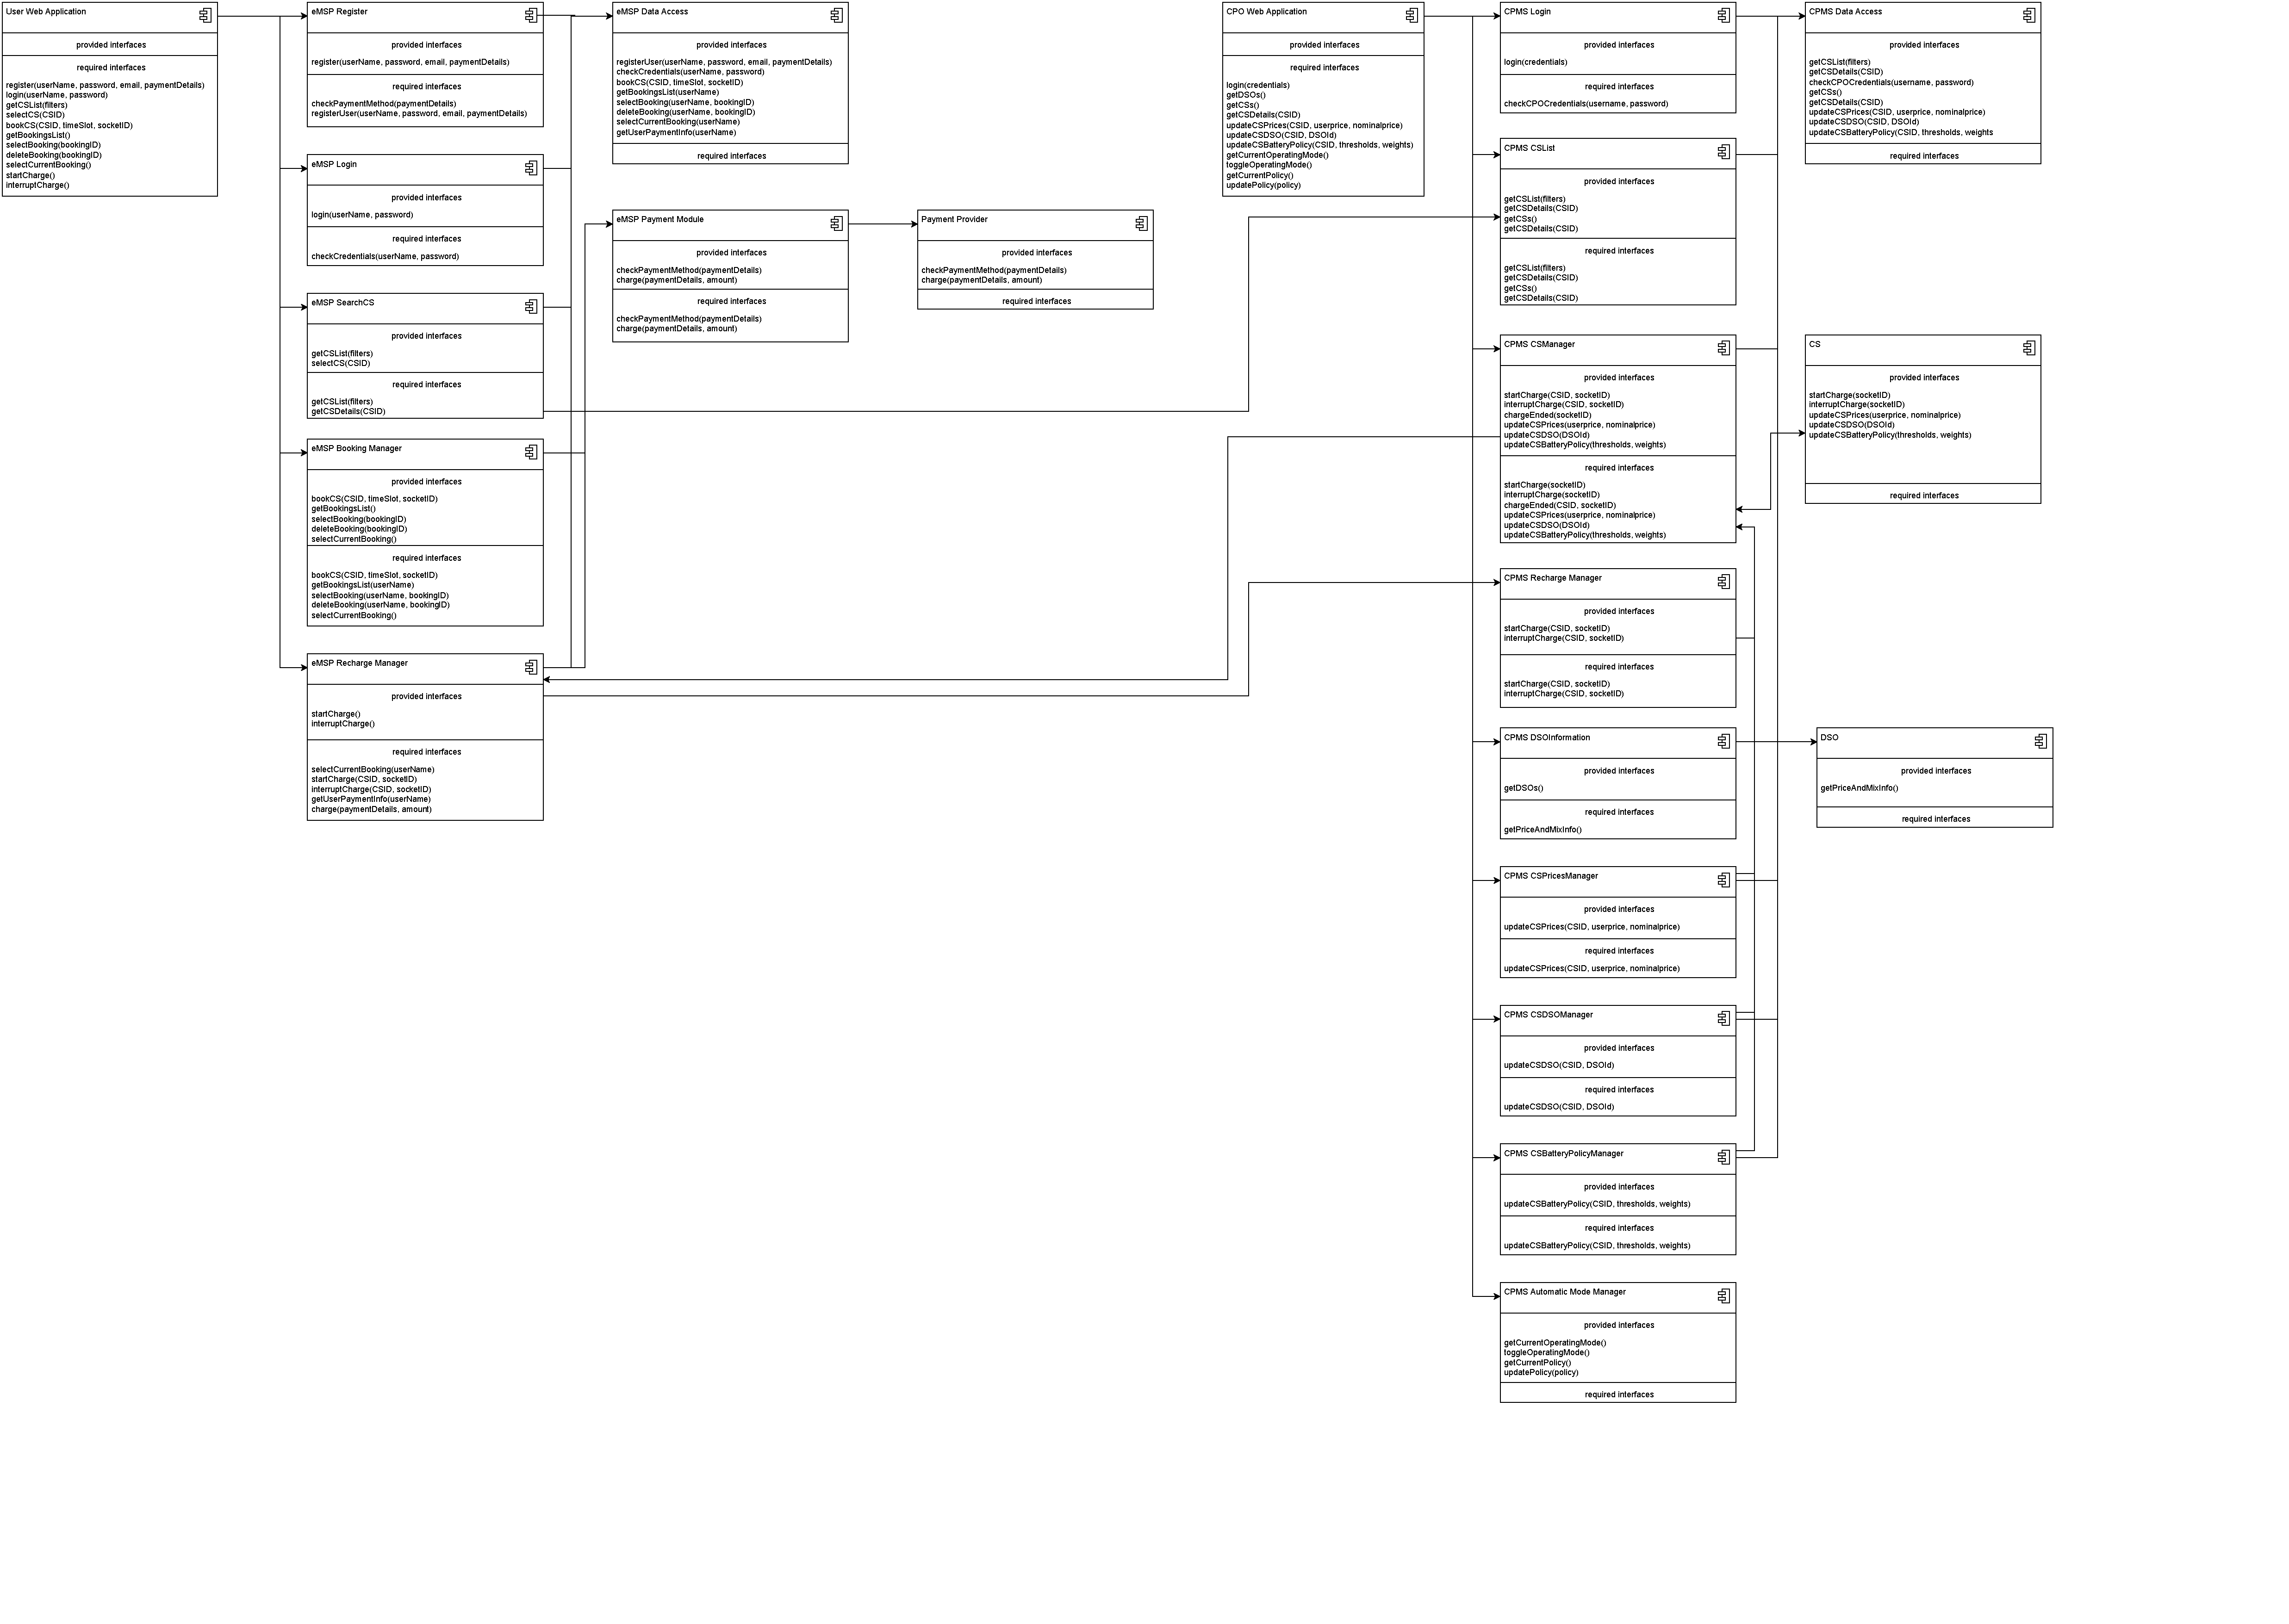
\includegraphics[page={1}, width=1.18\linewidth, trim=0cm 3.25cm 2cm 0cm, angle=-90, clip]{InterfacesDiagram.pdf}
    }
    \caption{Interfaces diagram}
\end{figure}

\newpage

\subsection{Selected Architectural Styles and Patterns}

Regarding architectural styles, both systems will use a \textbf{Client-Server} architecture, where clients can be both consumer-accessible devices (e.g. laptops, desktop PCs) or, as is the case for the CPMS, internal CS software. For communication, \textbf{REST APIs} are extensively used to expose a standard interface to all clients involved in the process, while adopting a de-facto industry standard for client-server communication. \\
To support the aforementioned client-server communication, the \textbf{HTTP} protocol is used, except for messages exchanged between the CSs and CPMS, which adopt the \textbf{WebSocket} protocol. \\
A \textbf{Model-View-Controller} approach is adopted for both the eMSP and CPMS infrastructures. The three components can be mapped as follows:
\begin{itemize}
    \item \textbf{View}: The Client-side HTML/CSS code, as well as JavaScript views used to present data to the user;
    \item \textbf{Controller}: The Client-side modules used to asynchronously request and send data to the back-end, but also the Server-side components handling all API routes;
    \item \textbf{Model}: Server-side representations of the data stored in the DB;
\end{itemize}
Therefore, the client can be classified as a \textbf{Fat Client}, since it incorporates part of the controller logic to handle asynchronous client-to-server communication and view updates. \\
This architectural style also maps easily to the \textbf{4-tier} architecture used by both systems, where the \textbf{Presentation Layer} includes both the \textbf{View} and part of the \textbf{Controller} (due to the fat client approach), the \textbf{Web Server} and \textbf{Application Server} run all the server-side \textbf{Controller} modules, as well as abstract \textbf{Model} representations, and the \textbf{DB Server} manages all the \textbf{Model} data. \\
Finally, the common \textbf{Observer} pattern is adopted for asynchronous events that require an action or a response by either a client or server. This pattern is employed mostly to handle CS event notifications, as well as for managing events such as a user skipping one of their bookings. \\

\subsection{Other Design Decision}

For security reasons, all passwords are never stored as clear text, but rather encoded using standard hashing algorithms (Ex: Bcrypt). \\
%If there is something to say about interactions with external stuff

\newpage

\section{User Interface Design}

The interface eMall will use is a web app, through which its Users will have available all \hyperref[subsec:prodfunctions]{product functions}. Such web app will need to be usable both on desktop and mobile devices, since a mobile device is what users will most likely have available to them while at the CS. \\
In order to allow the User to select an area of interest while searching for CSs, the user interface will make use of a map. \\
\\
What follows are some mockups for the eMSP's user interface design.

\begin{figure}[!ht]
    \centering
    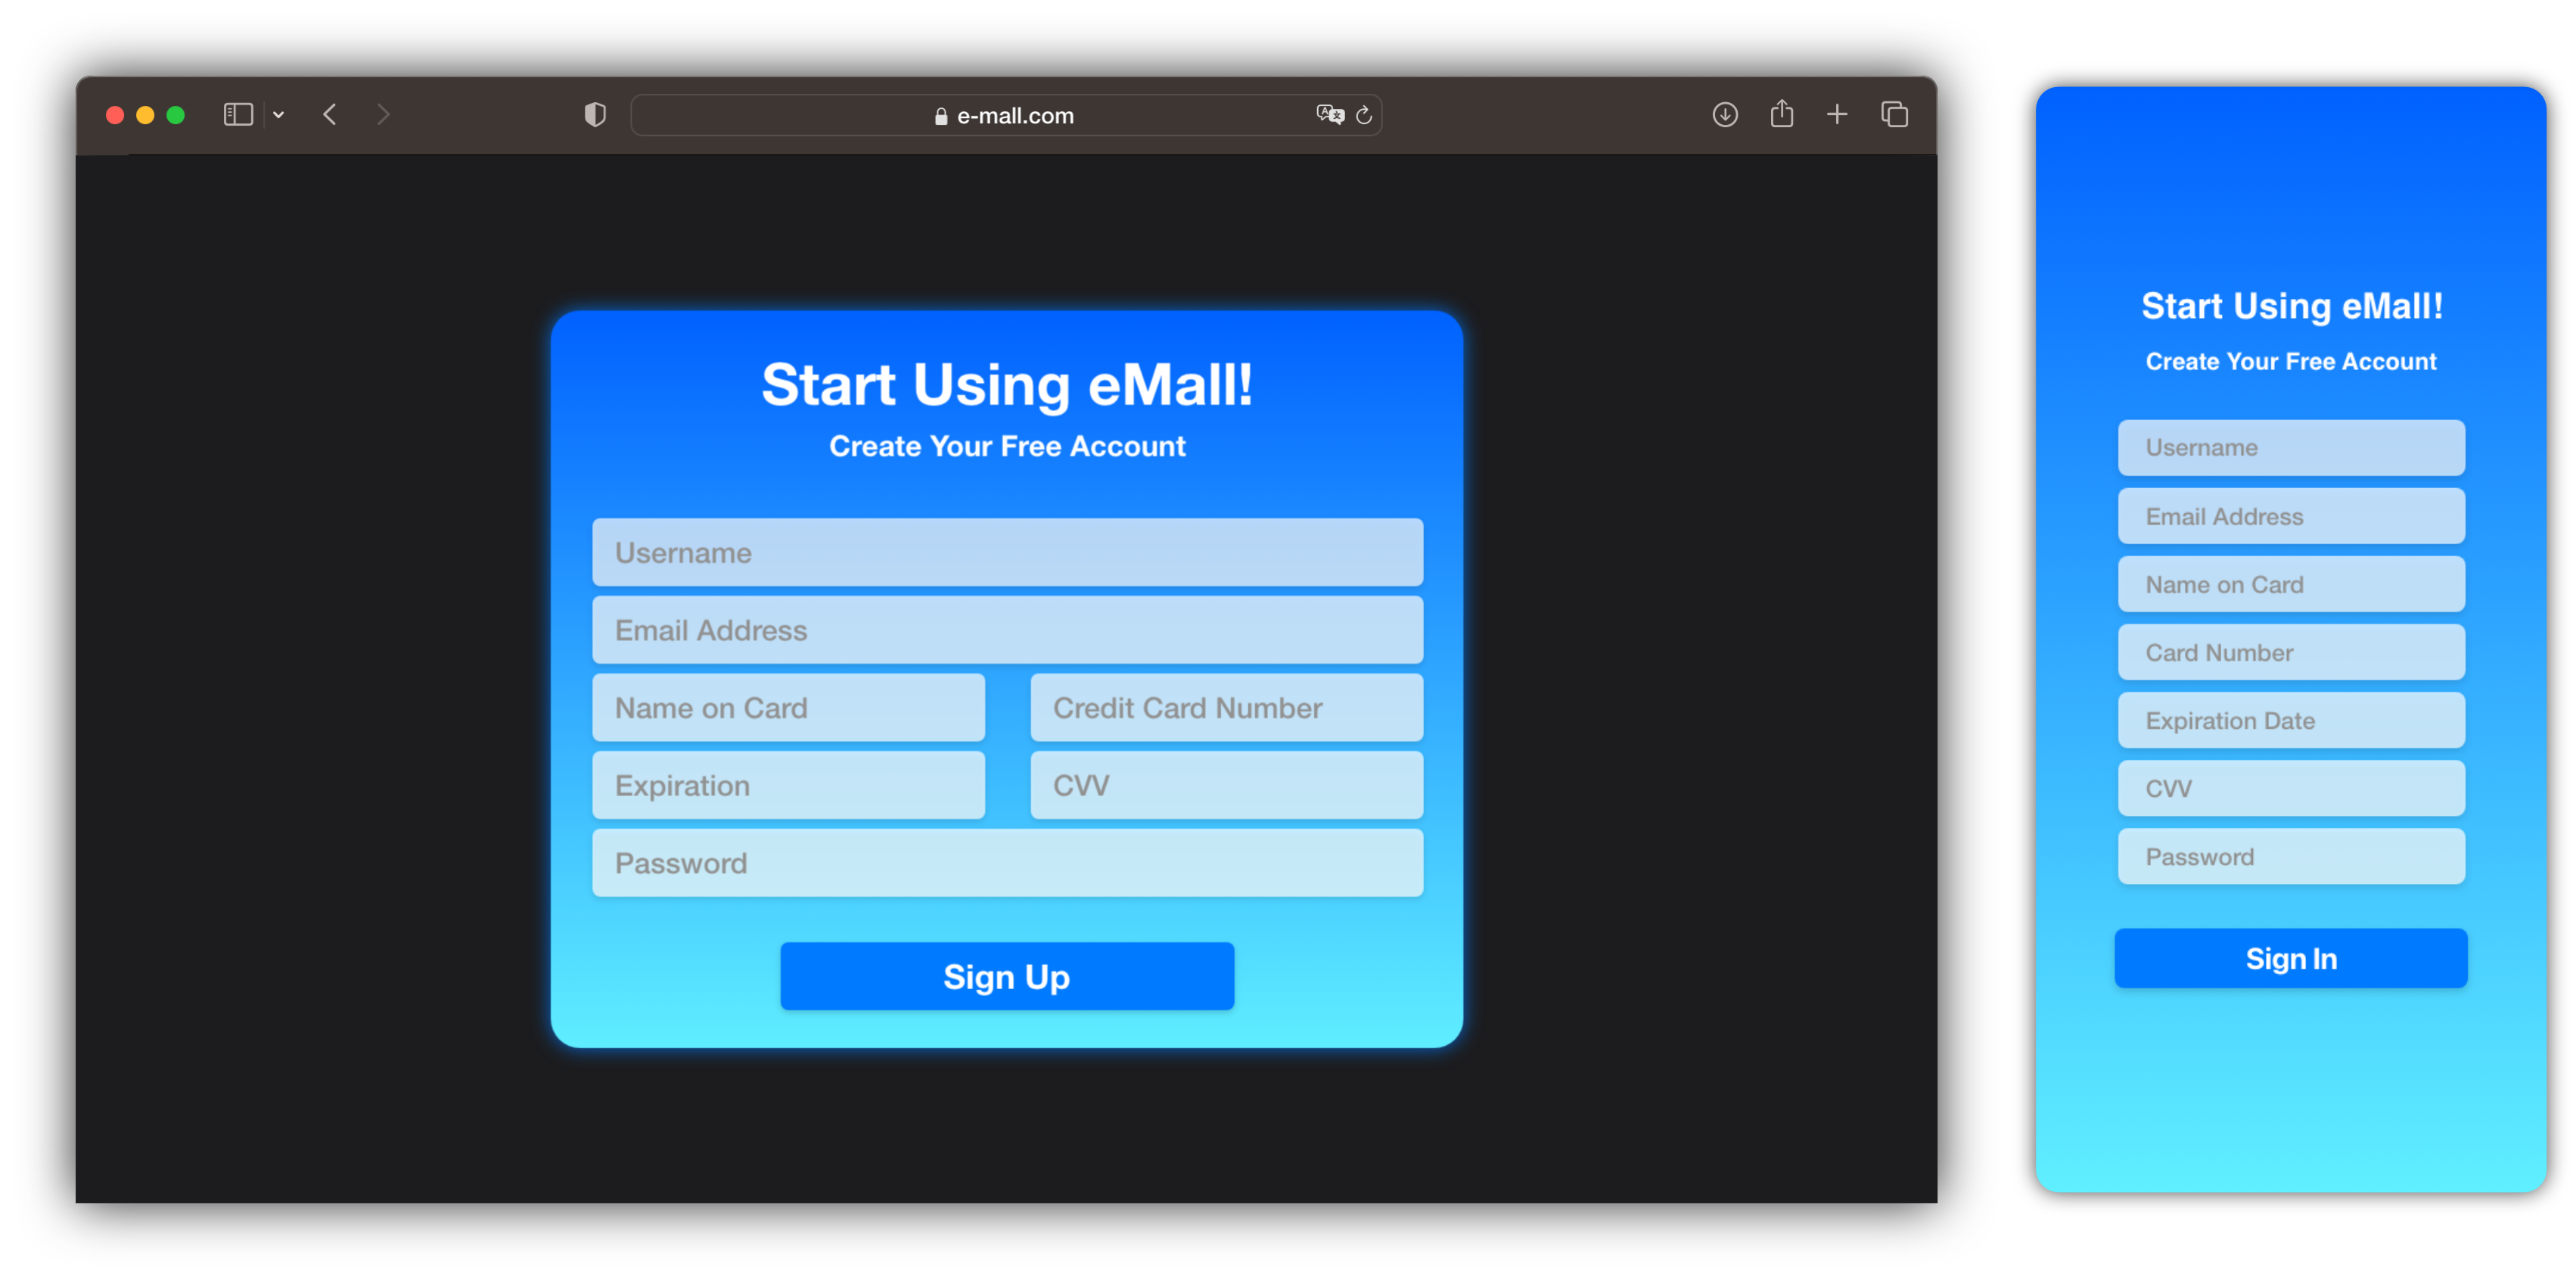
\includegraphics[width=180mm]{Signup.png}
    \captionsetup{justification=centering,margin=2cm}
    \caption{Signup page mockup \\
    %Is this enough of a description for ya?
    Users will be able to register into eMall by compiling the form with their data}
    \label{fig:my_label}
\end{figure}

\newpage

\begin{figure}[!ht]
    \centering
    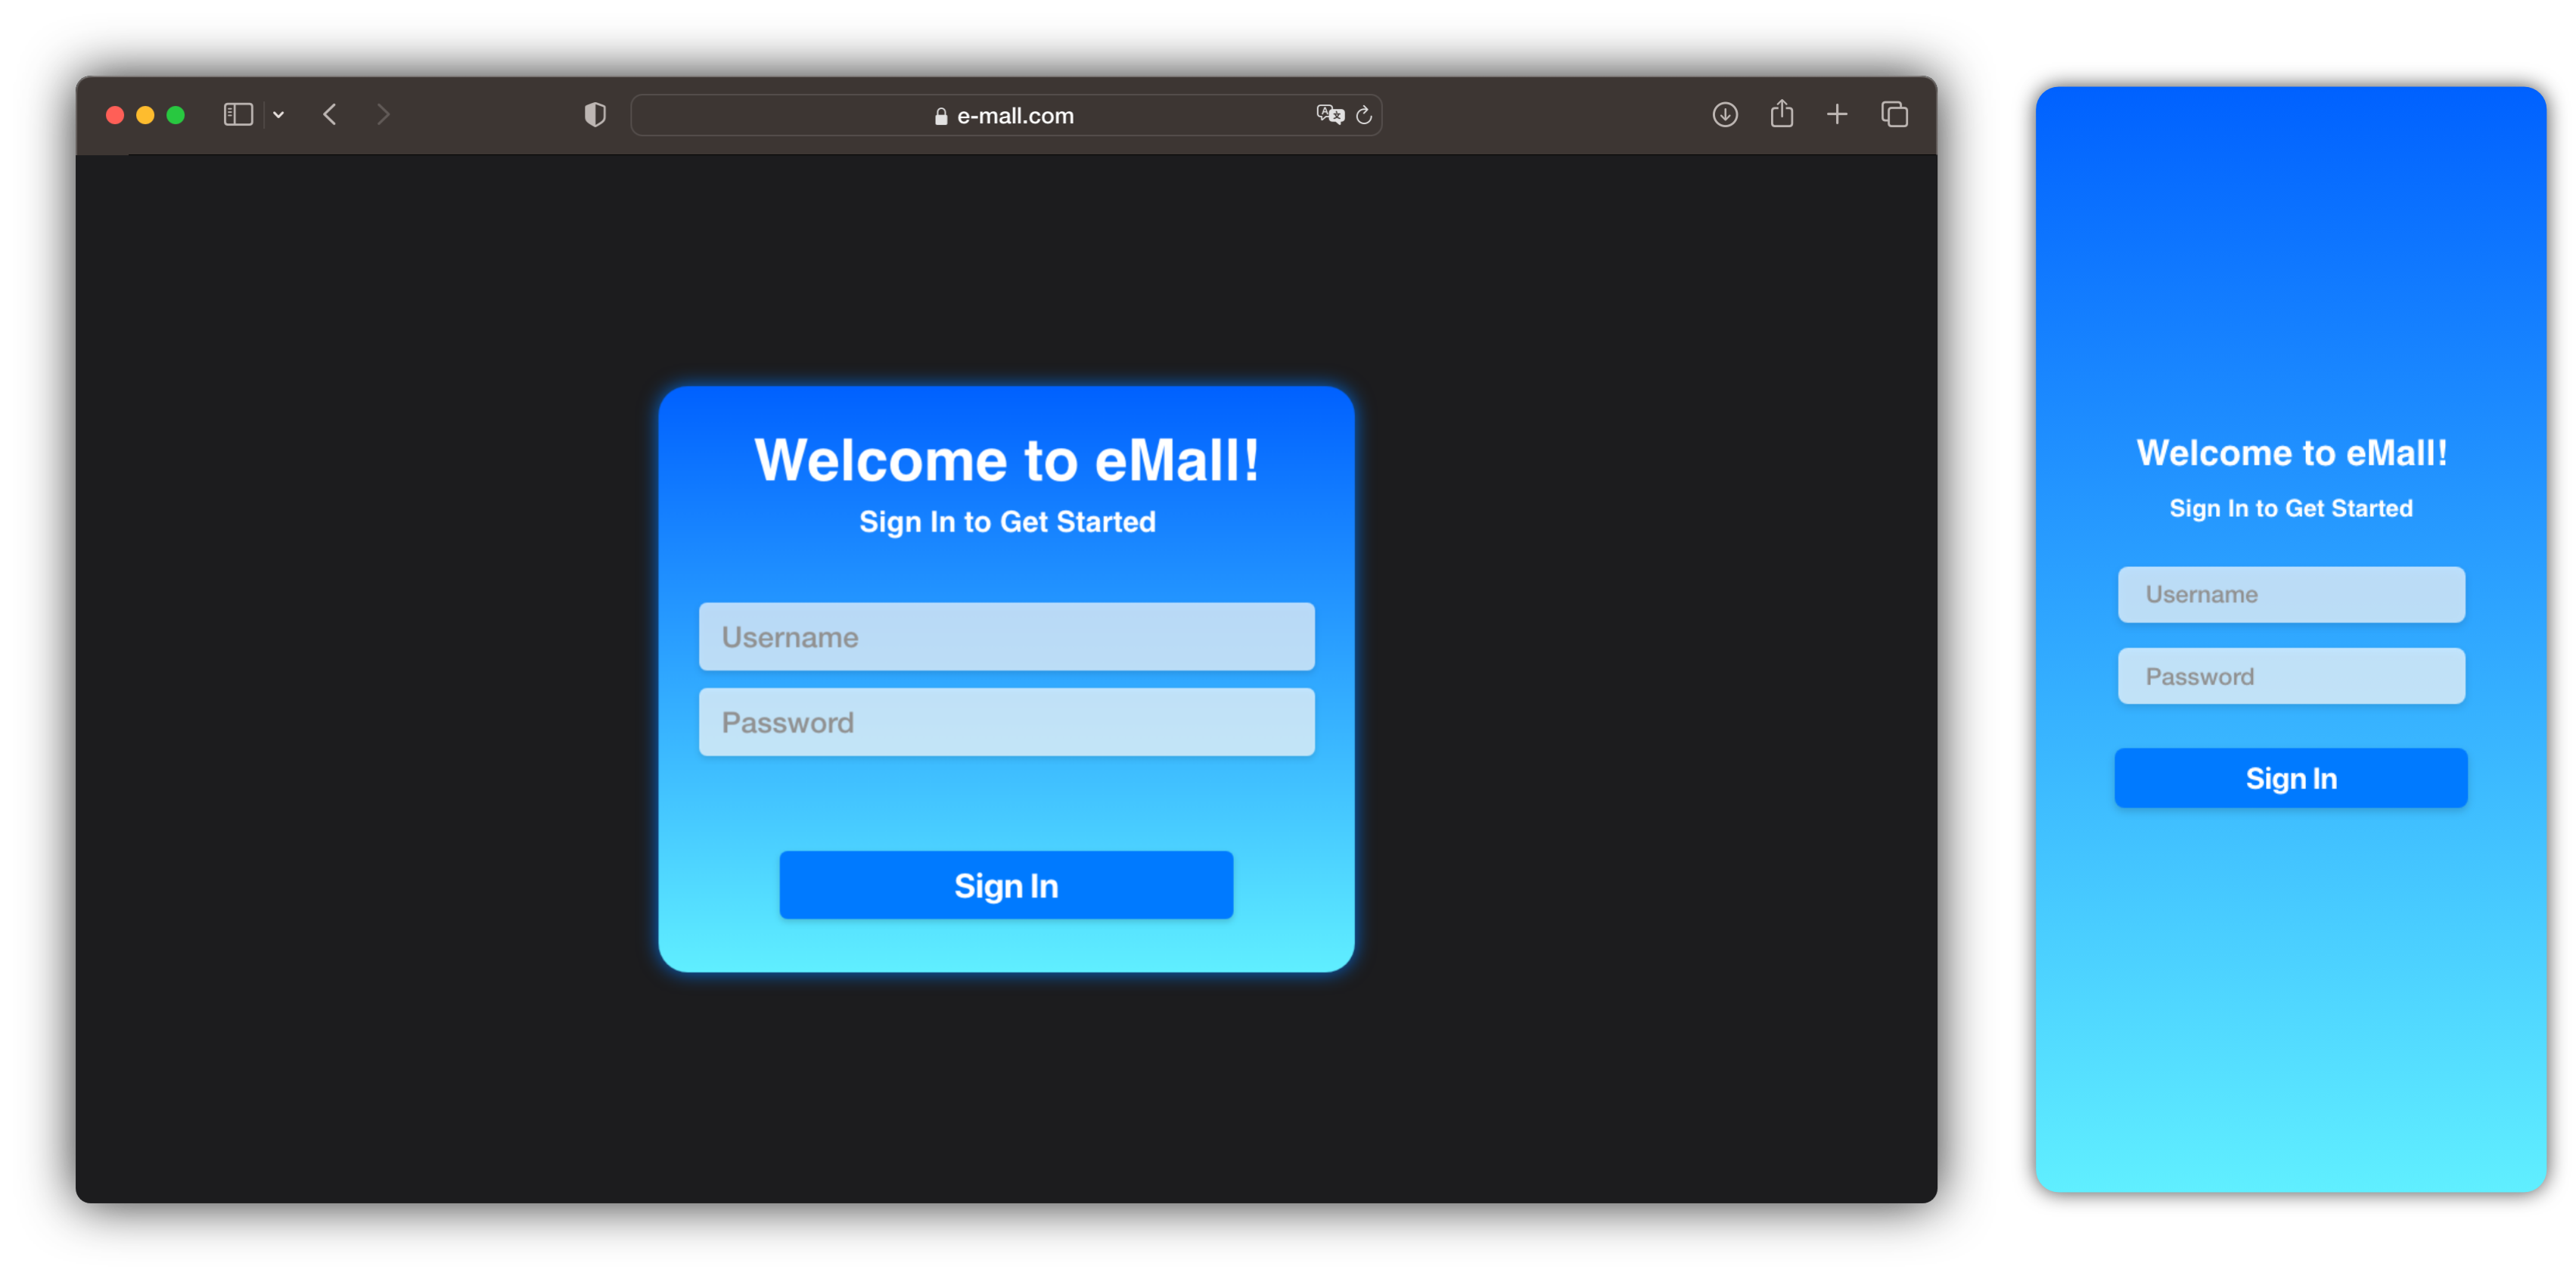
\includegraphics[width=180mm]{Login.png}
    \captionsetup{justification=centering,margin=2cm}
    \caption{Login page mockup \\
    Users will be able to log into their eMall account by inserting their credentials}
    \label{fig:my_label}
\end{figure}

\begin{figure}[!ht]
    \centering
    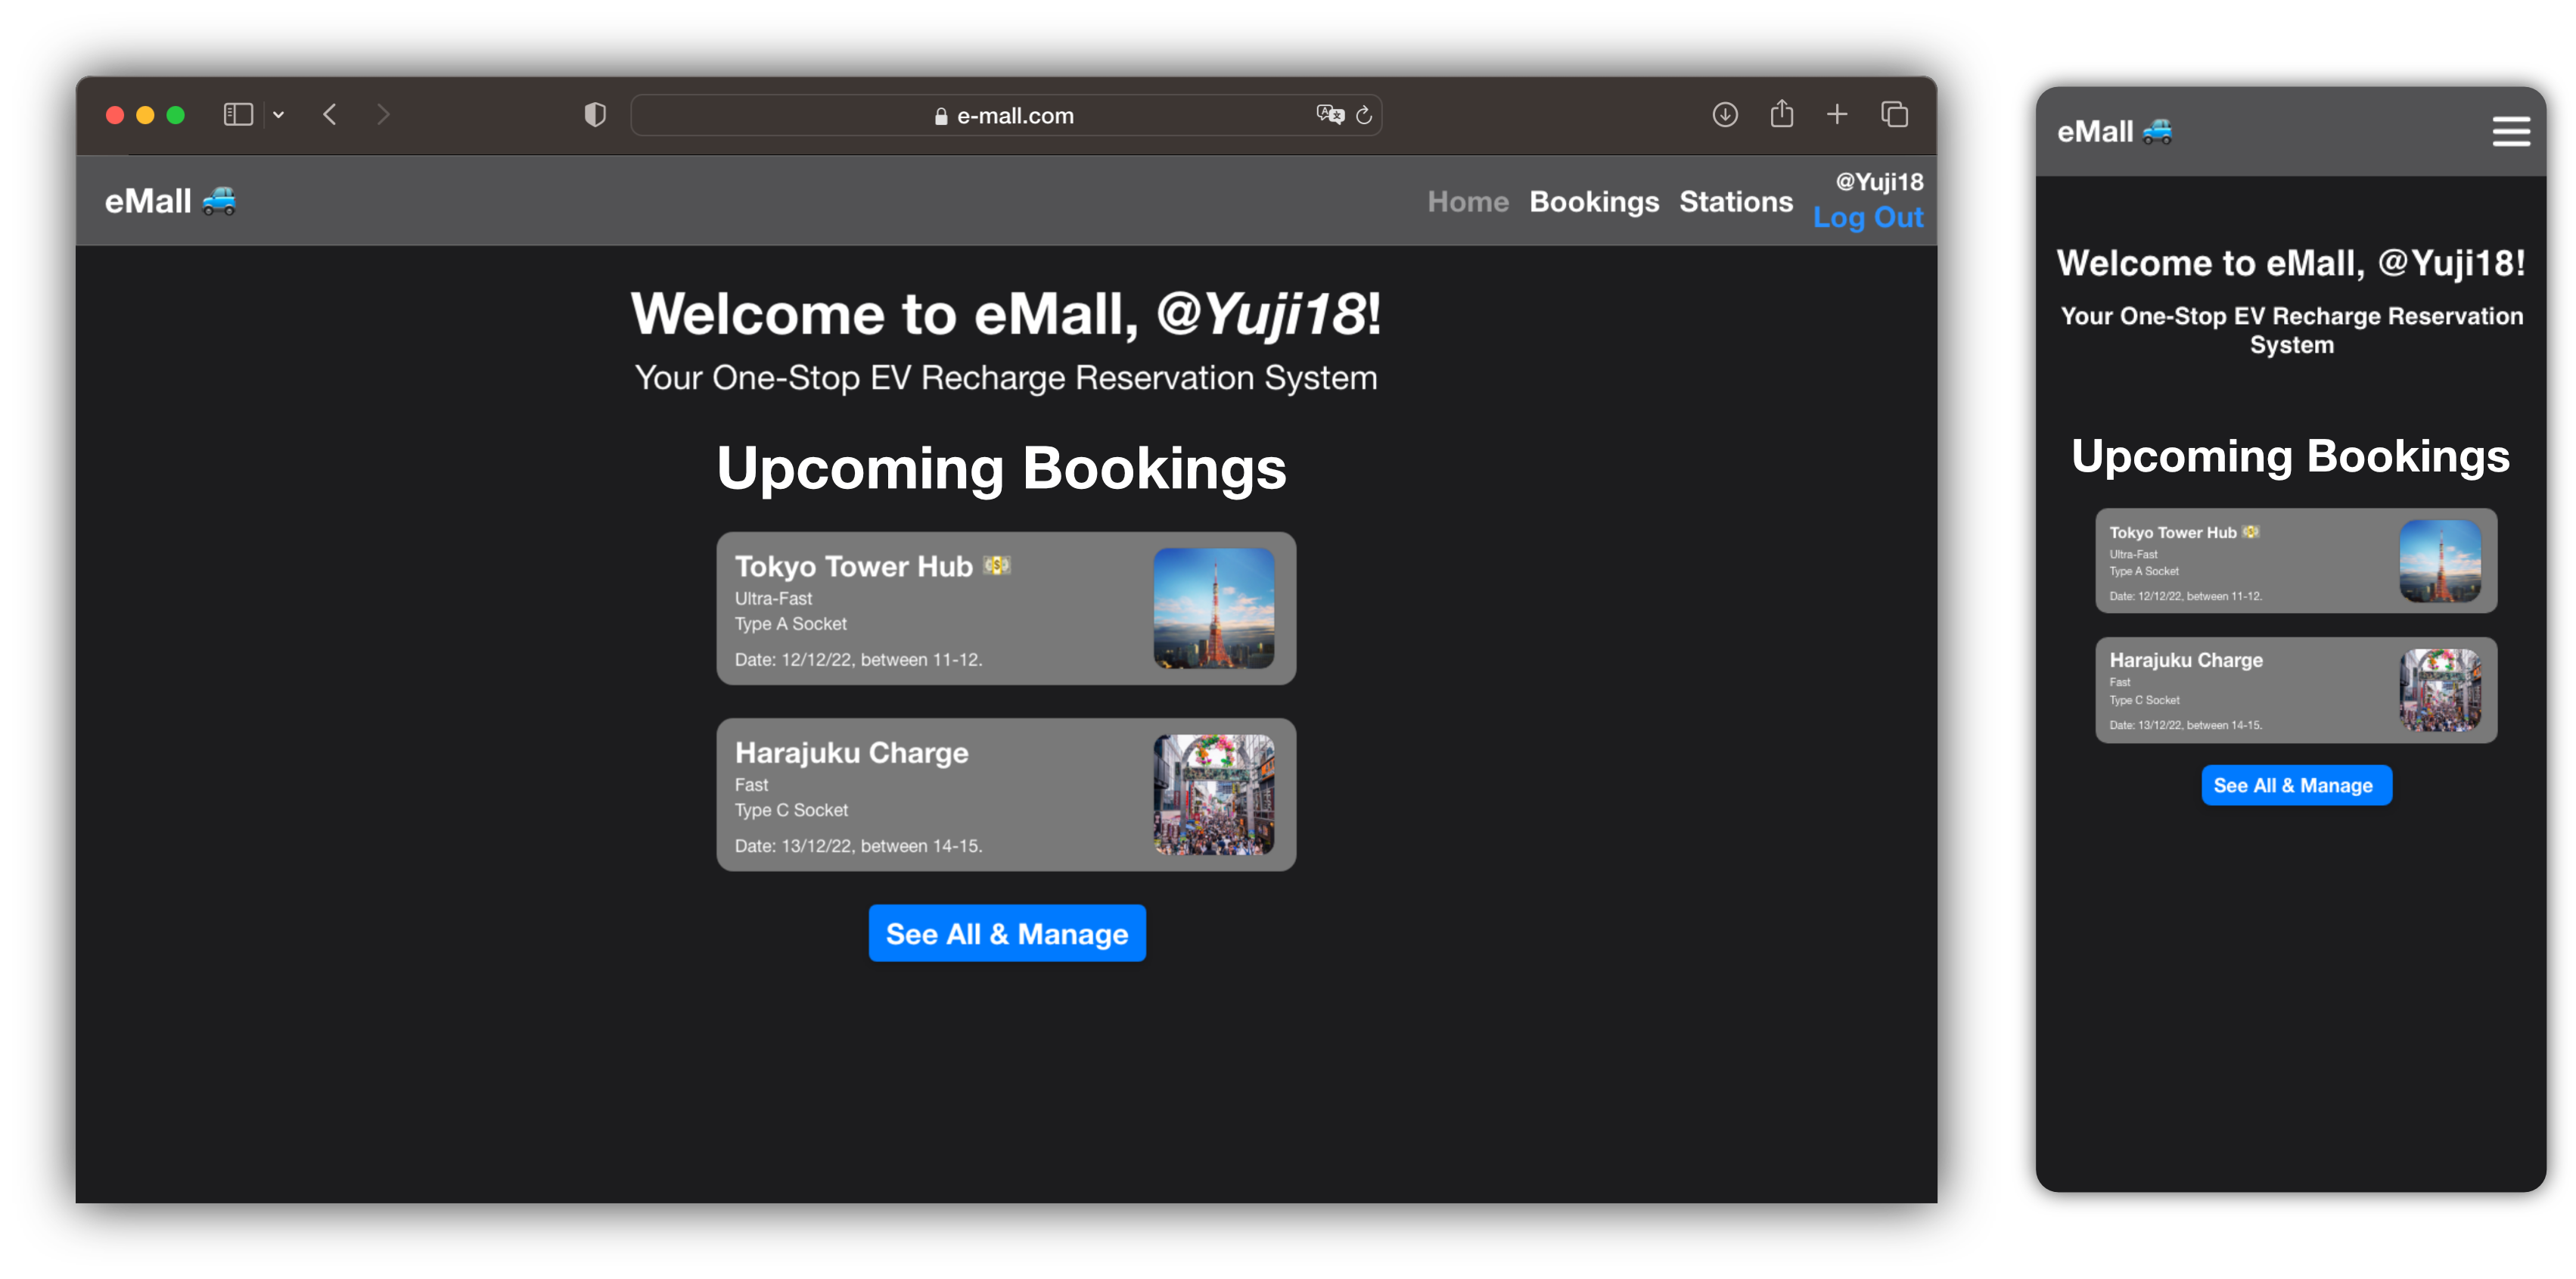
\includegraphics[width=180mm]{Home.png}
    \captionsetup{justification=centering,margin=2cm}
    \caption{Home page mockup \\
    Users will be able to click on the “See All” button to be redirected to the page with all their bookings}
    \label{fig:my_label}
\end{figure}

\newpage

\begin{figure}[!ht]
    \centering
    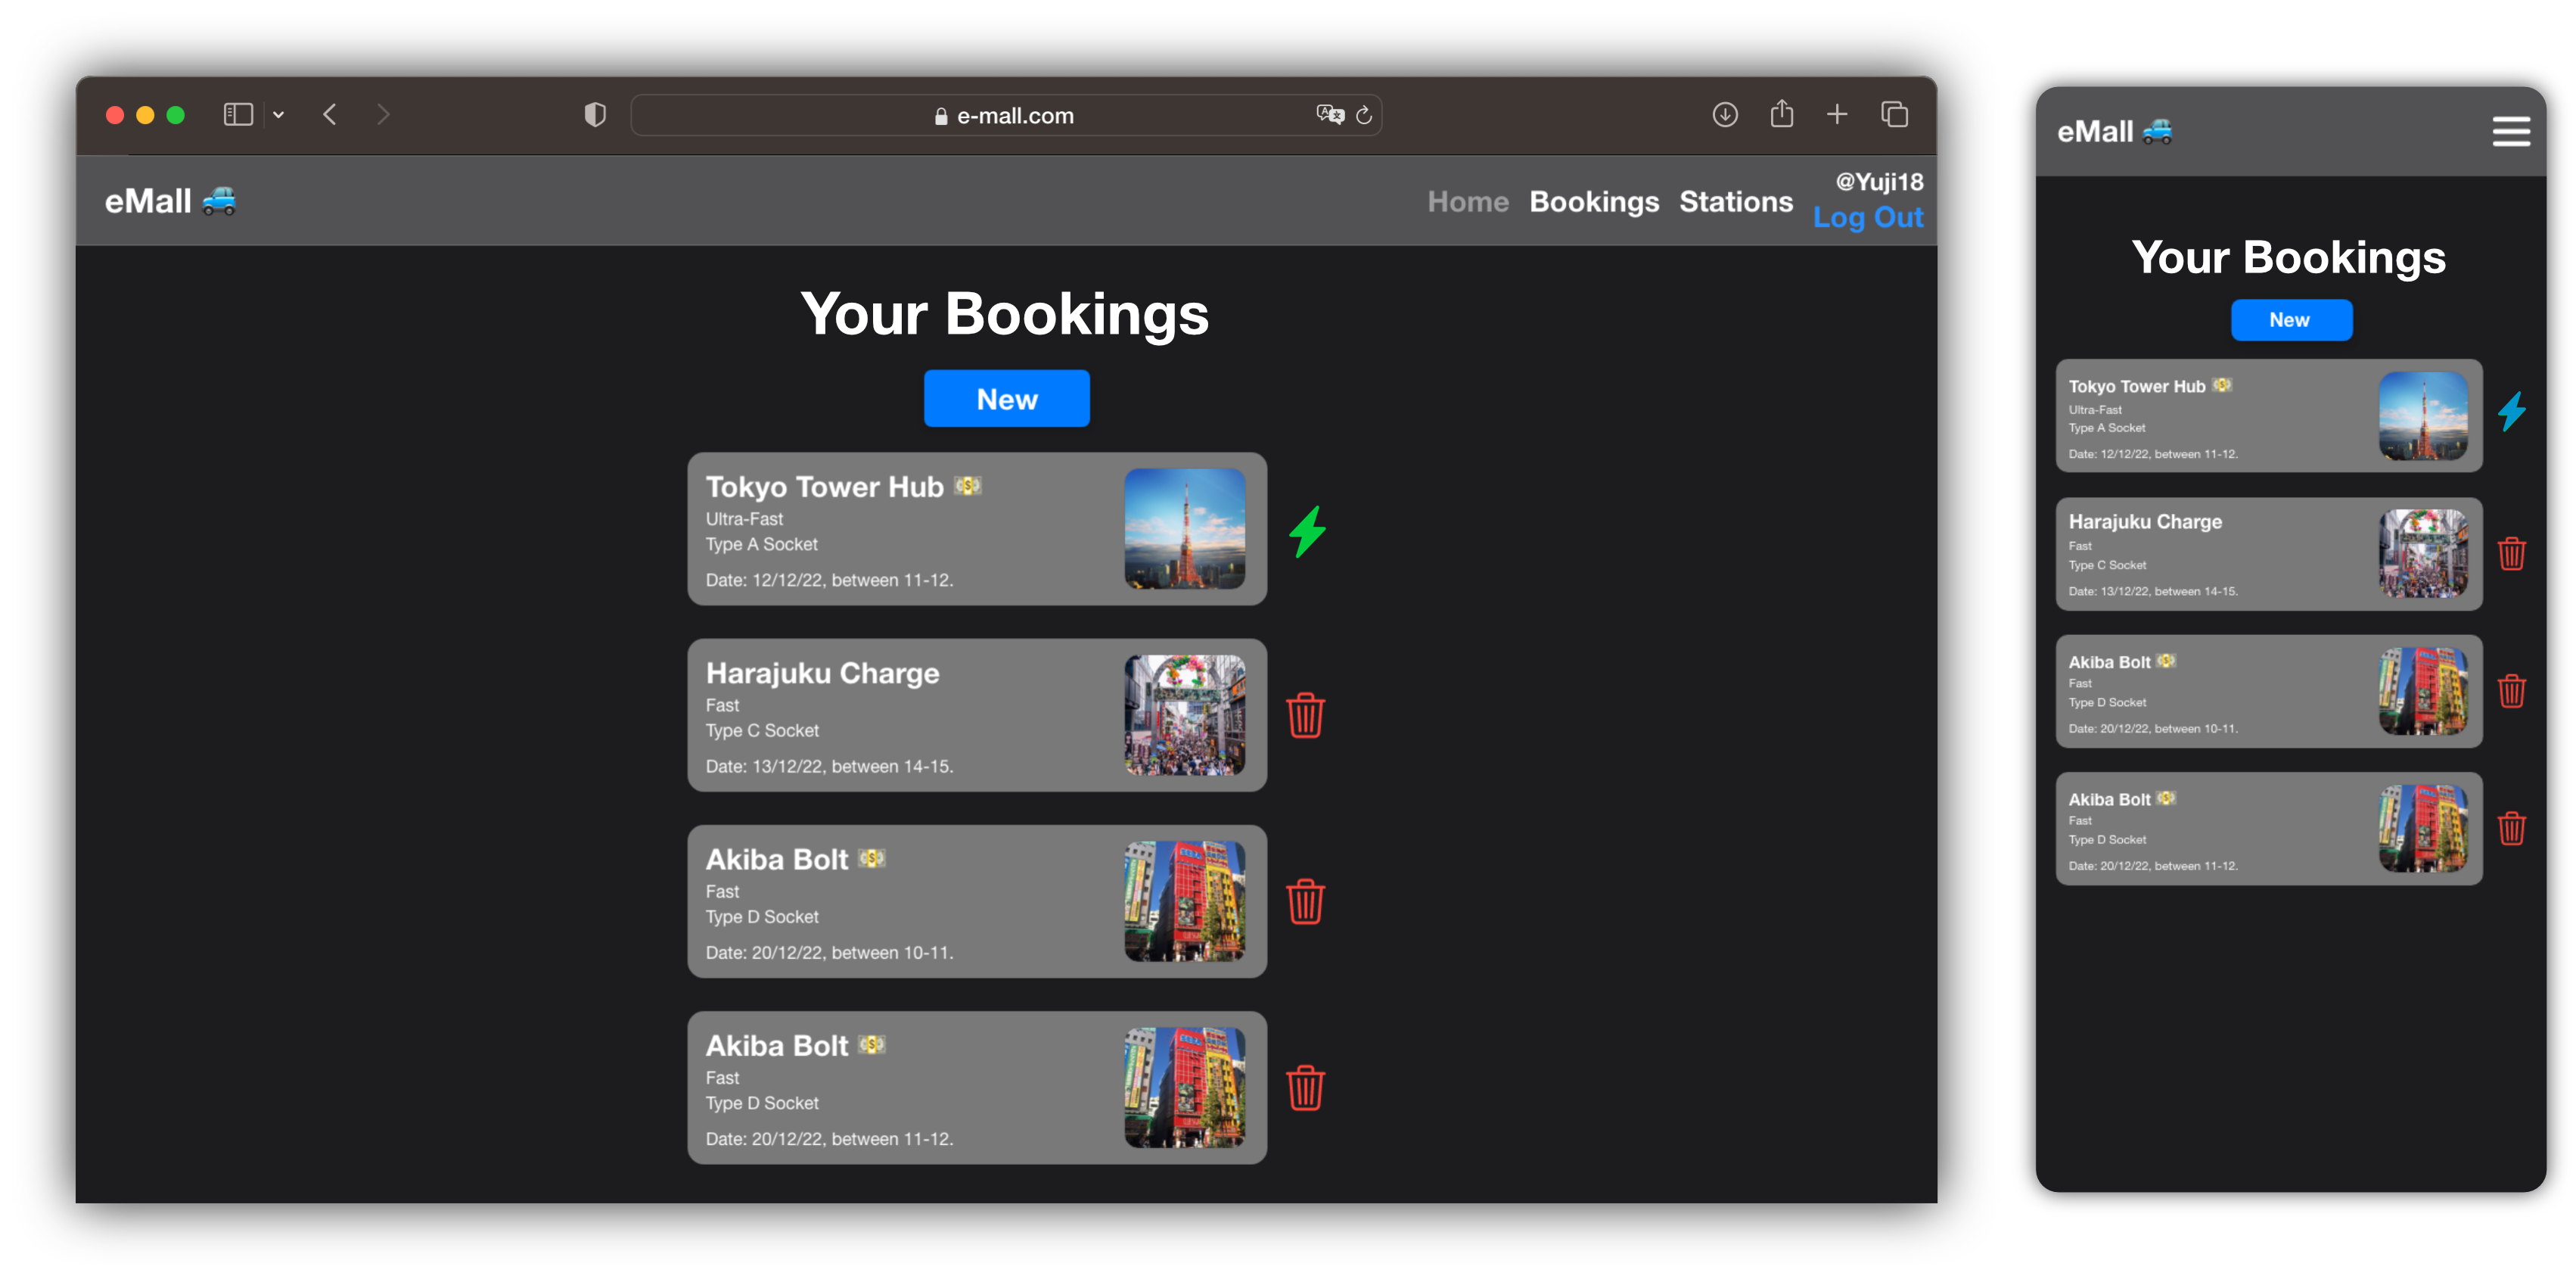
\includegraphics[width=180mm]{Bookings.png}
    \captionsetup{justification=centering,margin=2cm}
    \caption{Bookings page mockup \\
    Users will see the list of their bookings, with the option to delete any non-active one and to start their charge for any active booking with a vehicle connected}
    \label{fig:my_label}
\end{figure}

\begin{figure}[!ht]
    \centering
    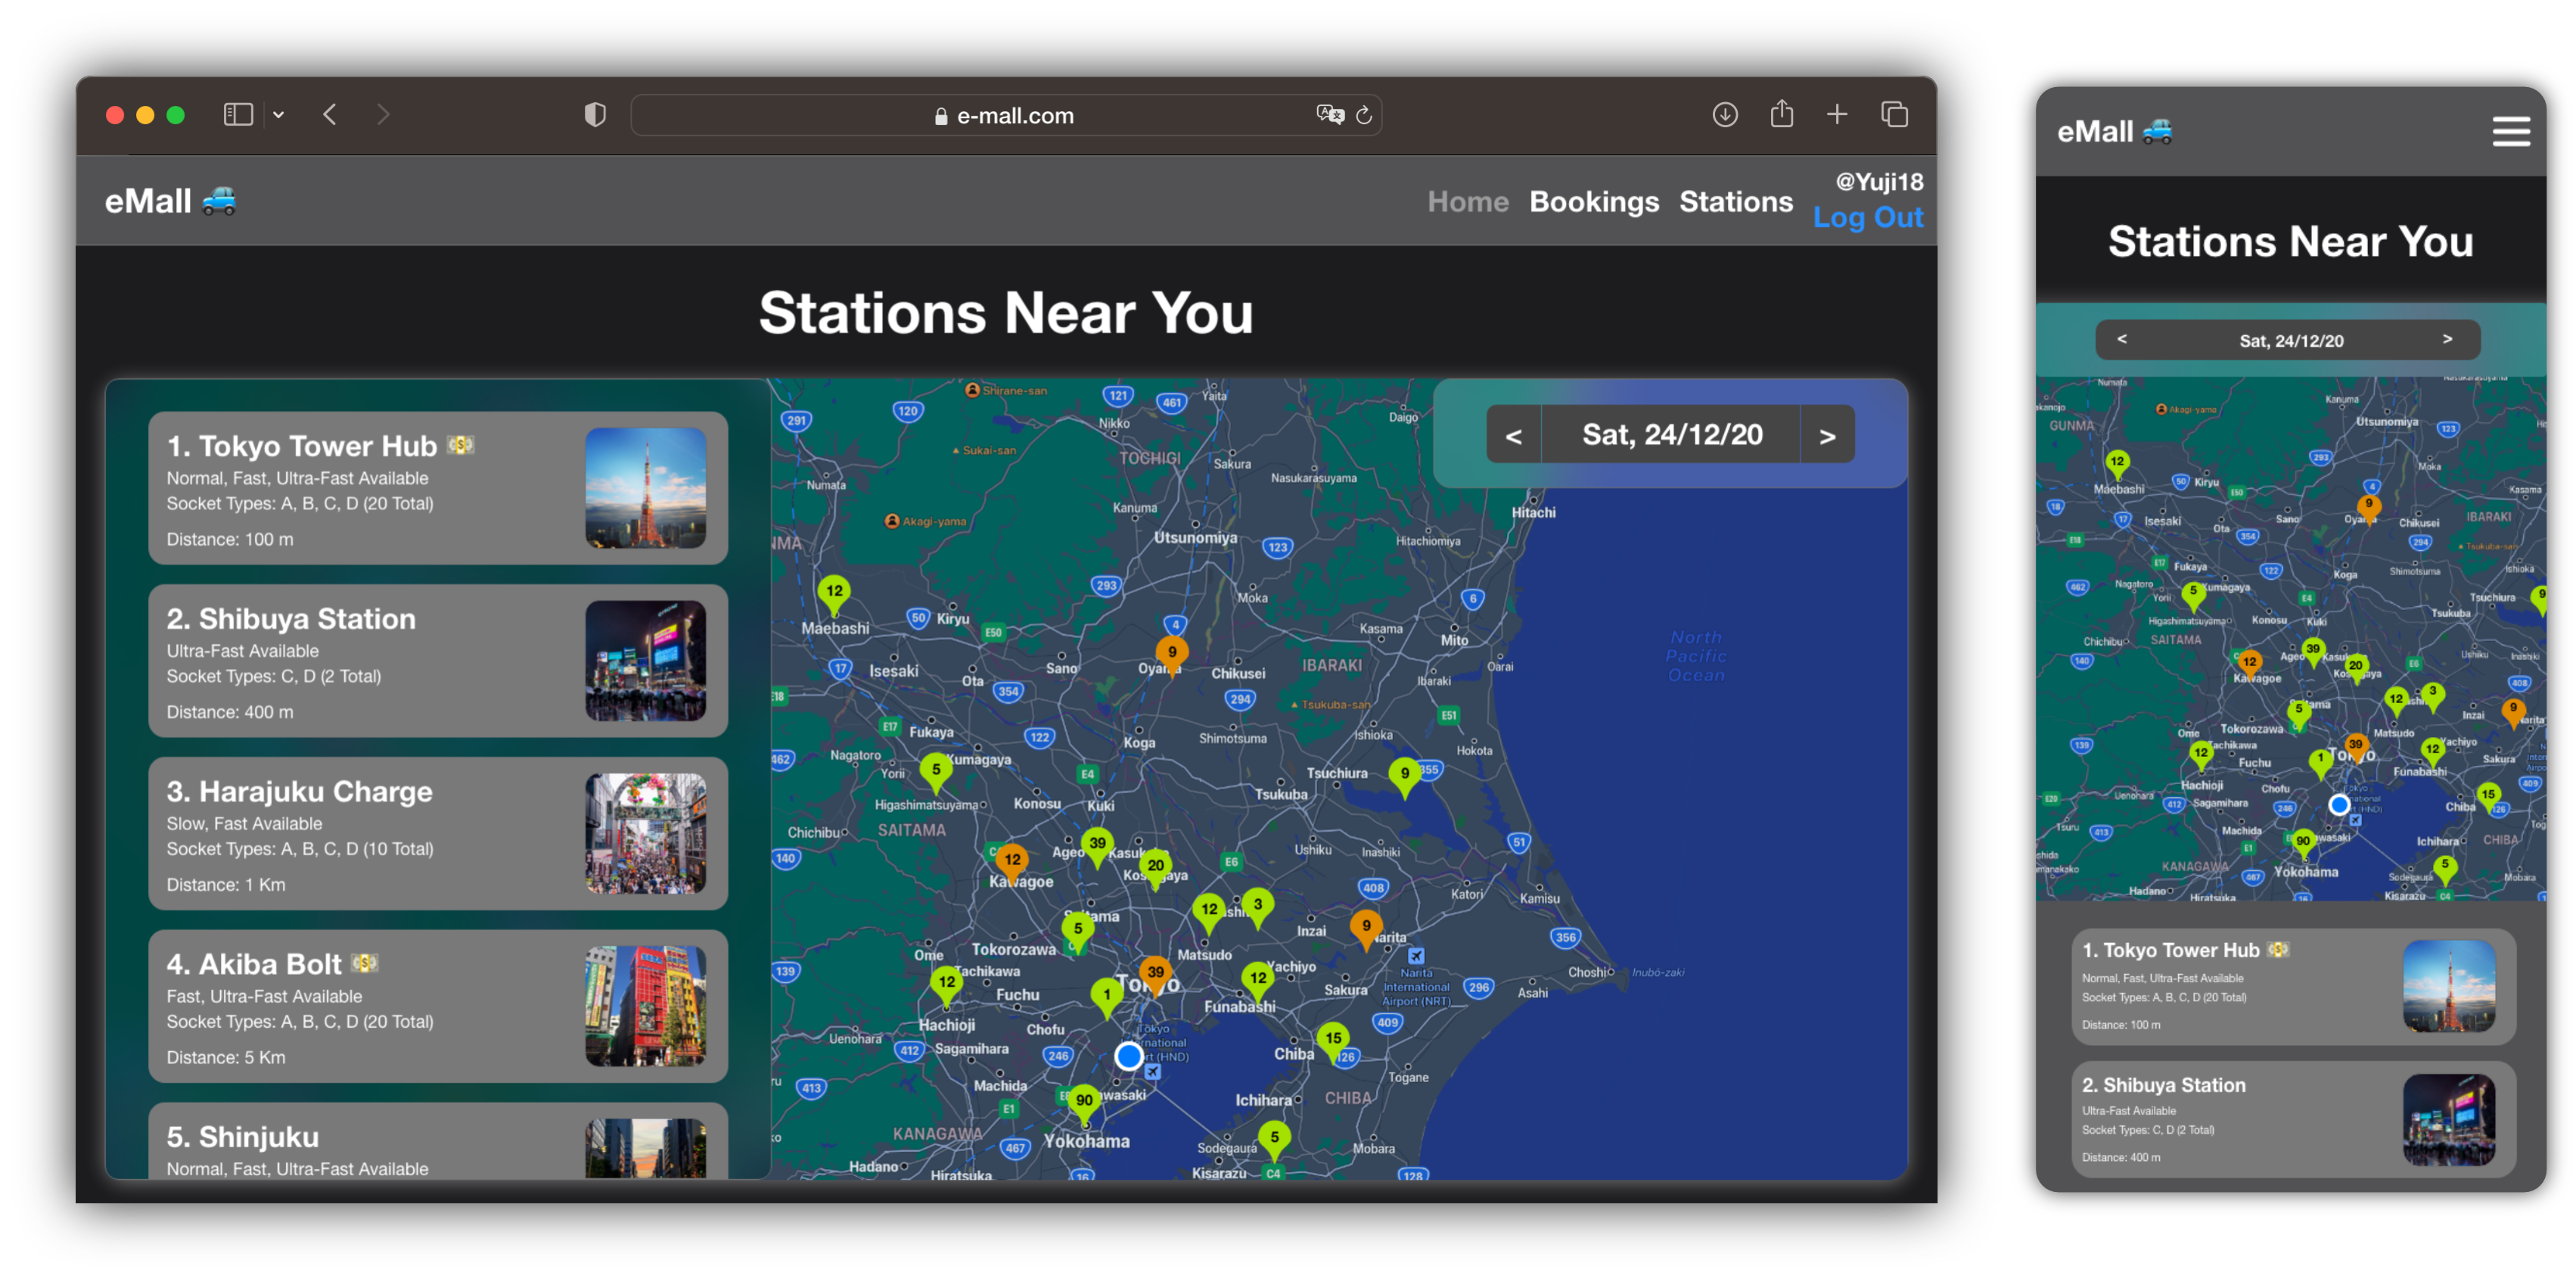
\includegraphics[width=180mm]{Stations.png}
    \captionsetup{justification=centering,margin=2cm}
    \caption{Stations page mockup \\
    Users can use the map together with the time selector to filter the search}
    \label{fig:my_label}
\end{figure}

\newpage

\begin{figure}[!ht]
    \centering
    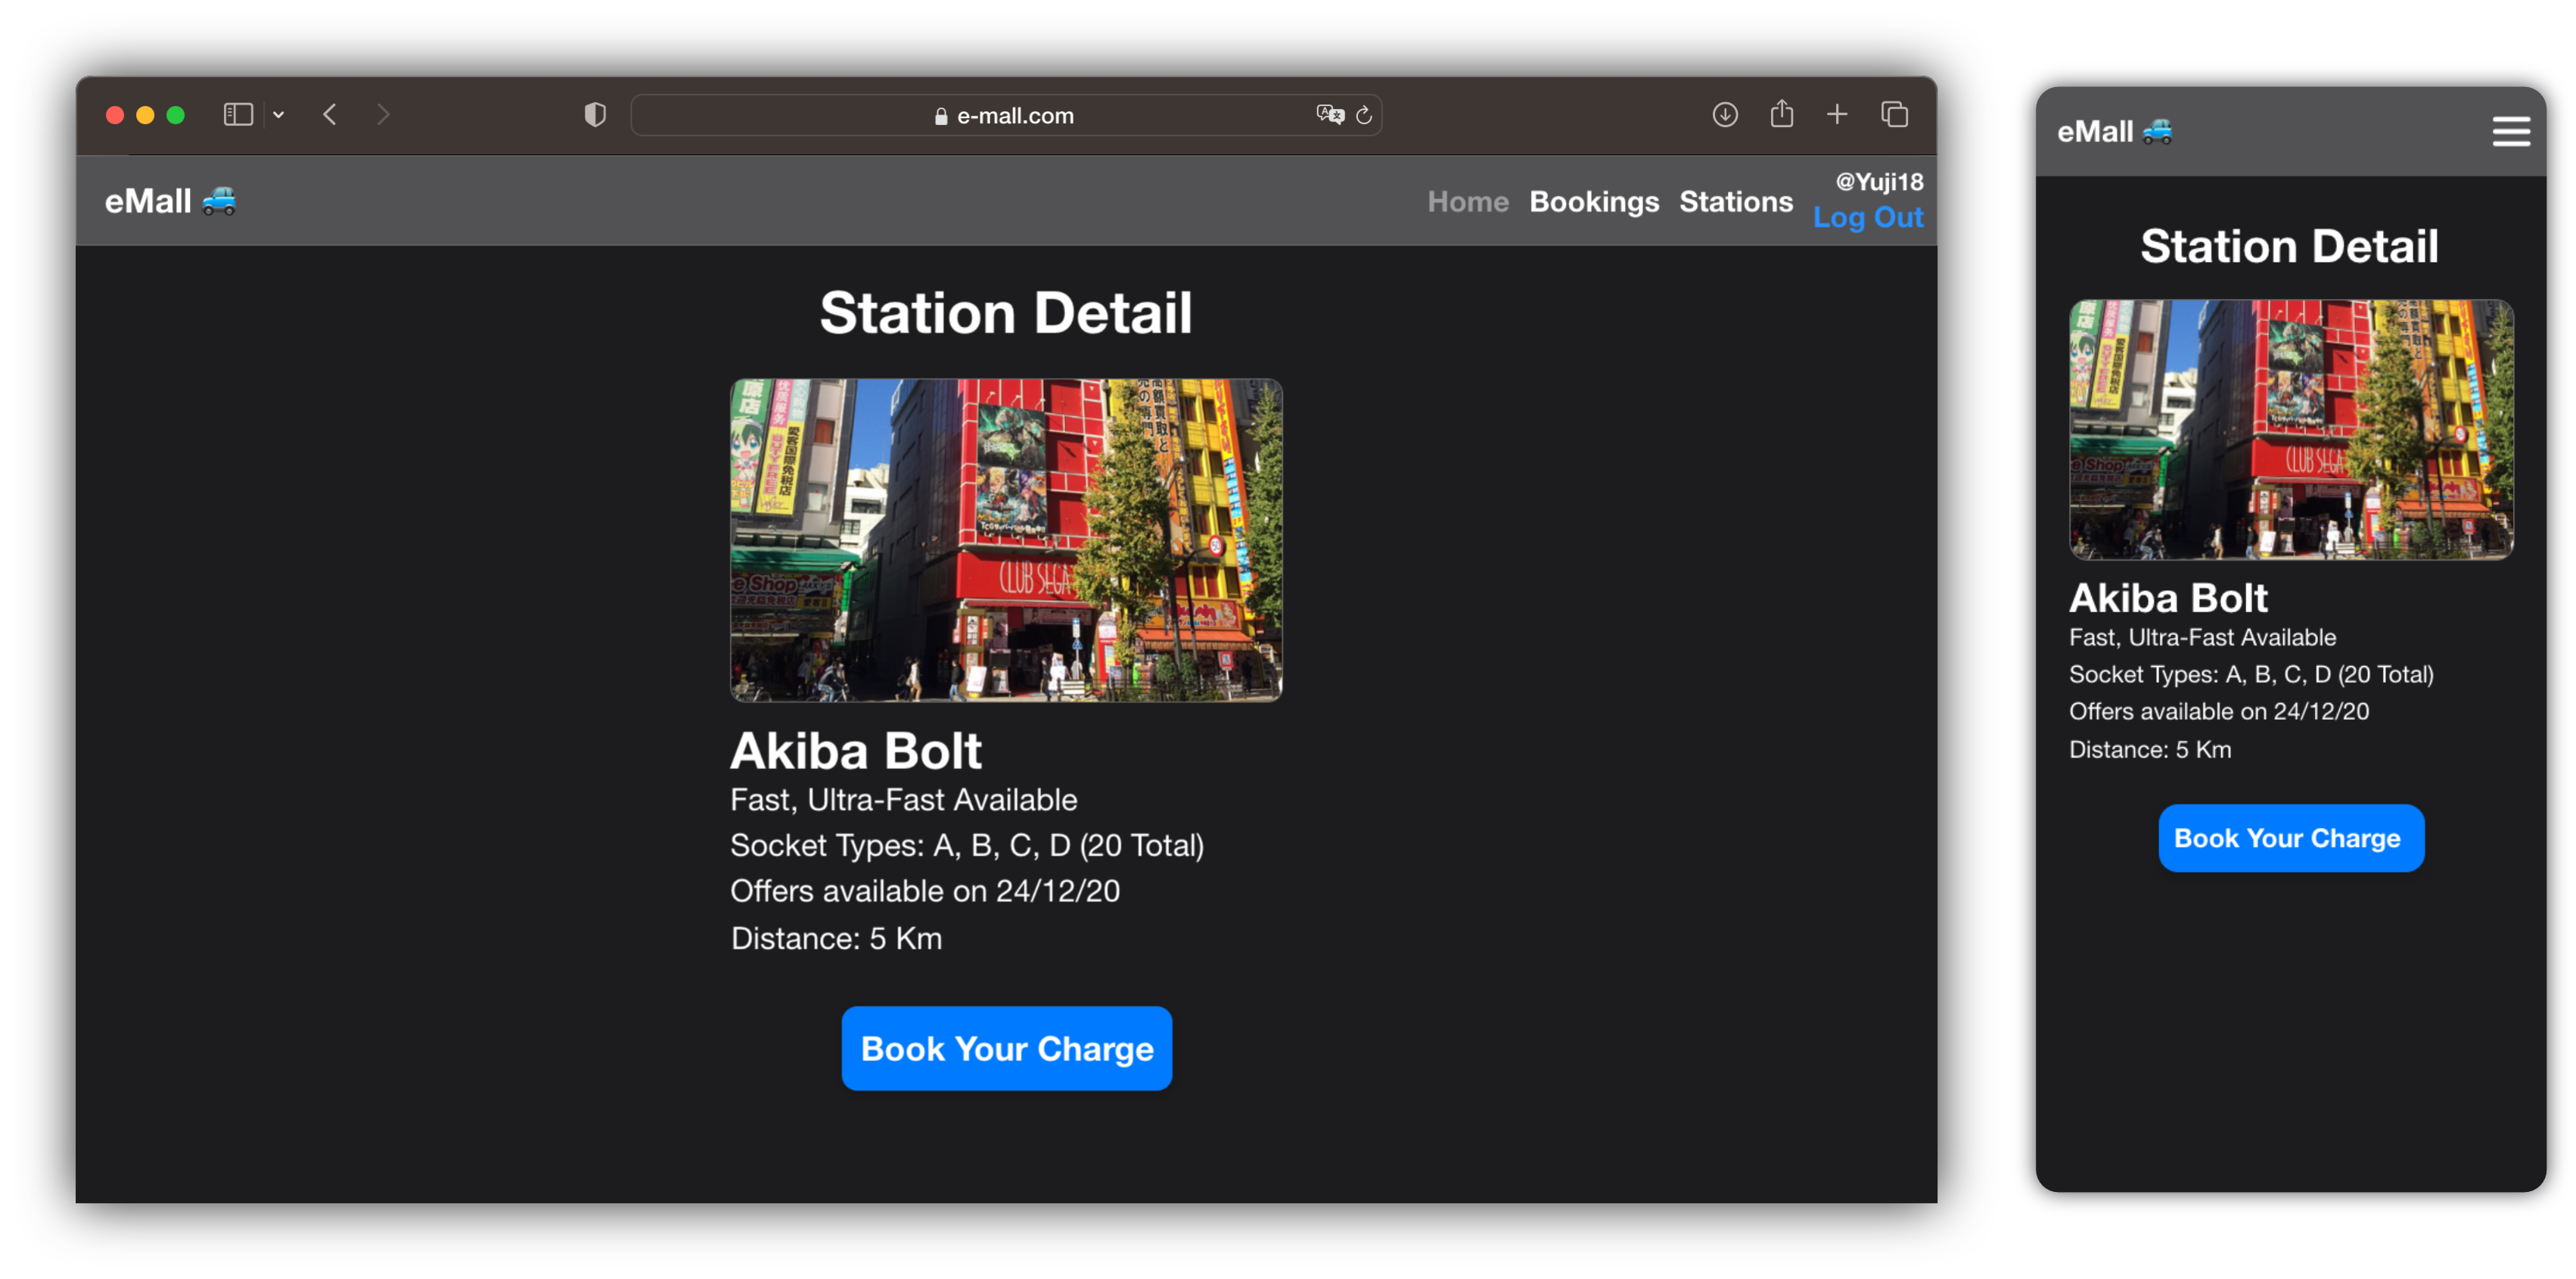
\includegraphics[width=180mm]{StationDetail.png}
    \captionsetup{justification=centering,margin=2cm}
    \caption{Station Details page mockup \\
    Users can click on “Book Your Charge” to open the page for booking creation}
    \label{fig:my_label}
\end{figure}

\begin{figure}[!ht]
    \centering
    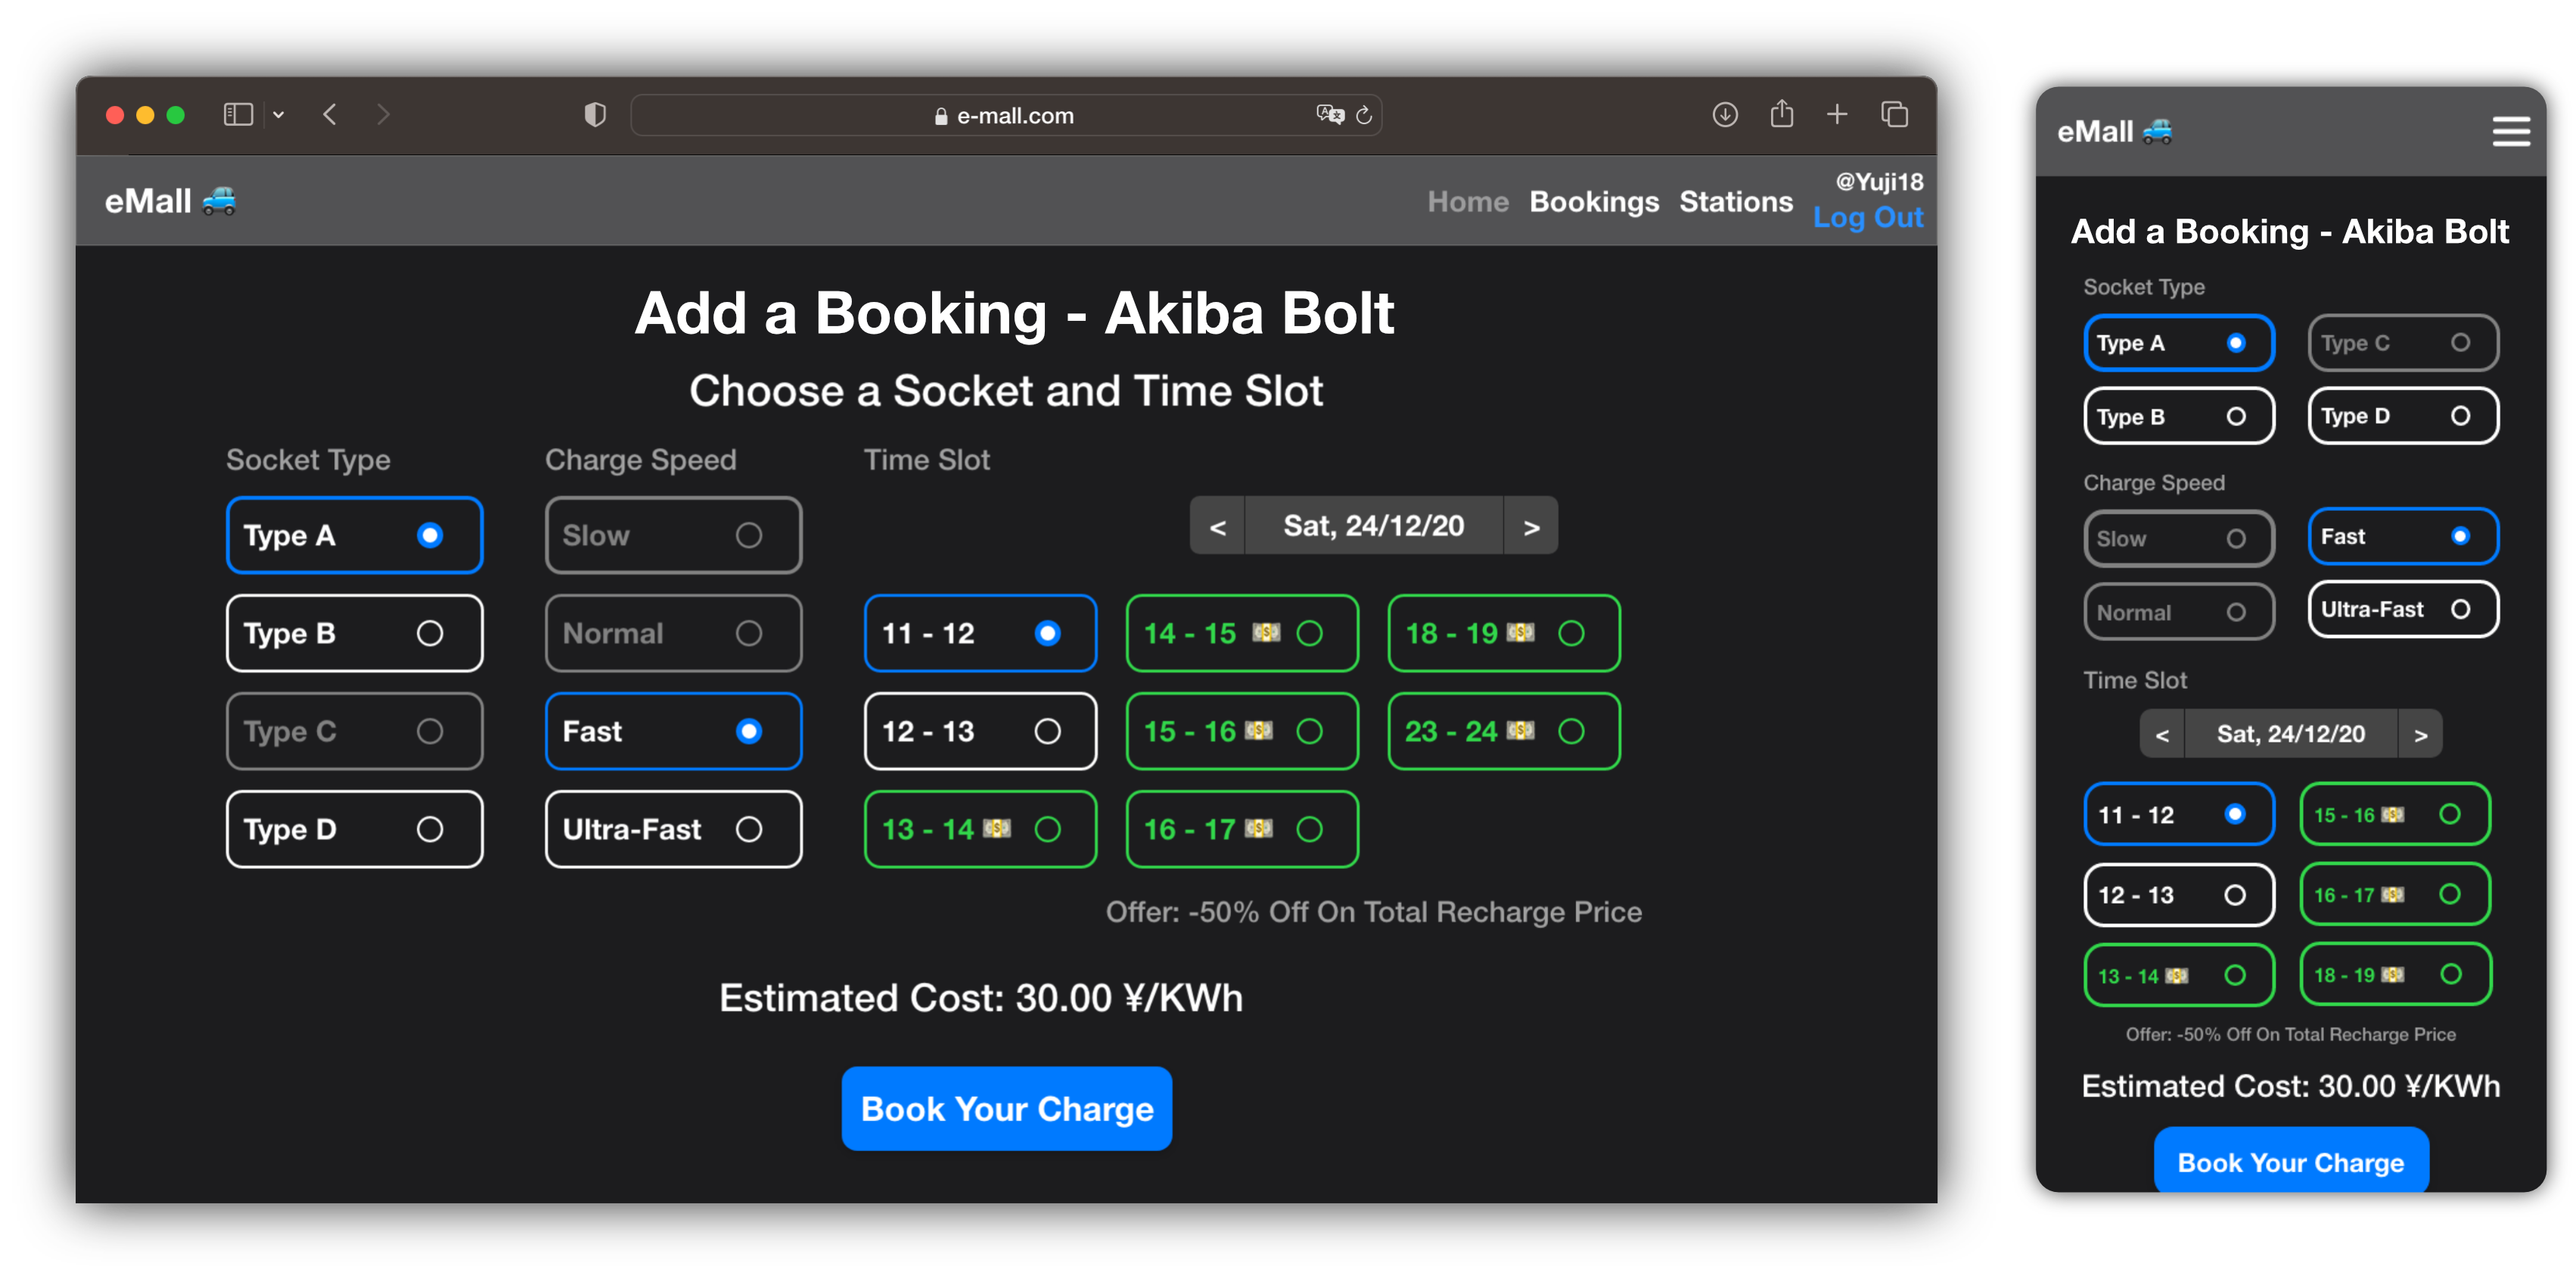
\includegraphics[width=180mm]{BookCharge.png}
    \captionsetup{justification=centering,margin=2cm}
    \caption{BookCharge page mockup \\
    Users can select the time slot for their booking as well as charge speed and socket type among the available ones}
    \label{fig:my_label}
\end{figure}

Similarly, CPMSs will offer their functionality to CPOs via a web portal, here there is no need to support anything other than a desktop device, since CPMSs are intended to be managed by employees in a company environment. Follow some mockups for the CPMS's user interface.

MOCKUPS HERE FOR CPMS!!!!

\newpage

\section{Requirements Traceability}

\section{Implementation, Integration and Test Plan}

Here we discuss how the architecture previously described will be realized, with its modules integrated and tested in order to guarantee the correctness of the final product, w.r.t. the requirements and directions expressed both in this document and the RASD, during each step of development.

\subsection{Implementation}

The implementation will proceed separately for the two main parts that the system is divided into, the eMSP and the CPMS, since the two can easily be implemented just by knowing the exposed interfaces of the other and no further knowledge. That being said, withing each part the implementation order can be the following:

\subsubsection{eMSP}

\begin{enumerate}
    \item The \textbf{Database} is the first component to implement as the way data is organized within it has to be reflected by the Data Access component.
    \item The \textbf{Data Access} component can be realized immediately after the DB, as it allows access from the other modules to the data it stores and is also relatively simple, mainly realizing ORM.
    \item The \textbf{Payment Module} as it is the gateway to interfaces with the Payment Provider, it needs to be implemented before the components which need access to the former.
    \item The following components can all be implemented concurrently as they have no dependencies with one-another and all constitute the interfaces which the Web Application relies upon.
    \begin{itemize}
        \item Login
        \item Register
        \item Serch CS
        \item Bookings Manager
        \item Recharge Manager
    \end{itemize}
    \item The \textbf{Authentication} component can be realized after the other back-end components, since all of them either rely on authenticated connections or grant them to clients, but only the request router uses this component to verify the session of a connected client.
    \item The \textbf{Web Application} is realized for last as it is the less critical component and its testing can be highly aided by the existence of all the other back-end components. To be noted that the Web Application's UI design, not its functionalities, can be realized at any time, while the development of the application is bonded to this sequence.
\end{enumerate}

\subsubsection{CPMS}

\begin{enumerate}
    \item The \textbf{Database} is the first component to implement as the way data is organized within it has to be reflected by the Data Access component.
    \item The \textbf{Data Access} component can be realized immediately after the DB, as it allows access from the other modules to the data it stores and is also relatively simple, mainly realizing ORM.
    \item The \textbf{CS Manager} is a critical component that needs to be realized before the others as it handles communications with the CSs and offers the functionalities that allow other components to configure CSs.
    \item The following components can all be implemented concurrently as they have no dependencies with one-another, they either expose and API for the CPO's web application or an API intended for the eMSP. 
    \begin{itemize}
        \item Login
        \item CS Battery Policy Manager
        \item CS DSO Manager
        \item CS Prices Manager
        \item Automatic Mode Manager
        \item CS List
        \item Recharge Manager
        \item DSO Information
    \end{itemize}
    \item The \textbf{Authentication} component can be realized after the other back-end components, since all of them either rely on authenticated connections or grant them to clients, but only the request router uses this component to verify the session of a connected client.
    \item The \textbf{Web Application} is realized for last as it is the less critical component and its testing can be highly aided by the existence of all the other back-end components. To be noted that the Web Application's UI design, not its functionalities, can be realized at any time, while the development of the application is bonded to this sequence.
\end{enumerate}

\subsection{Integration and Testing}

In this section we present our integration and testing plan for both systems. Since the two systems are designed to be distinct, they are first tested separately, following two parallel bottom-up approaches while stubbing the CPMS (for the eMSP) and writing a driver of the eMSP (for the CPMS). After all tests have been carried out (that is, all unit tests and bottom-up integration testing) the final integration of the two systems is carried out by removing stubs and drivers and using the pre-defined interfaces for communication between the two parties. \\
As hinted above, the two systems will use the following testing plan:
\begin{enumerate}
    \item \textbf{Unit Testing} of each component;
    \item \textbf{Bottom-Up Integration Testing} with appropriate drivers;
    \item \textbf{Final Integration Testing} by removing the CPMS stub (on the eMSP side) and the eMSP-like driver (on the CPMS side)
\end{enumerate}
This plan allows for easier bug identification and fixing, and ensures that whenever a component is finished its behavior is fully compliant with all the requirements. \\
It should be noted, however, that some components must be assumed to work as expected, since they are external modules that cannot be tested. An example of this is the DBMS, which is stubbed in all unit tests. \\
In addition, a variety of System Tests are used to ensure that properties of the system as a whole are respected. In particular, the following tests are adopted:
\begin{itemize}
    \item \textbf{Functional Testing}, to make sure that each requirement specified in the RASD document has been implemented properly;
    \item \textbf{Performance Testing}, to analyze key metrics of the performance of the system (such as response time) and identify and remove possible bottlenecks that would hamper the user experience;
    \item \textbf{Stress Testing}, to ensure that the system remains stable even under heavy or unforeseen load conditions.
\end{itemize}
Below is a list of diagrams illustrating the bottom-up integration testing approach and how all modules are progressively integrated and tested together. \\

\subsubsection{eMSP Integration}

%trim = left bottom right top 
\begin{figure}[!ht]
    \centering
    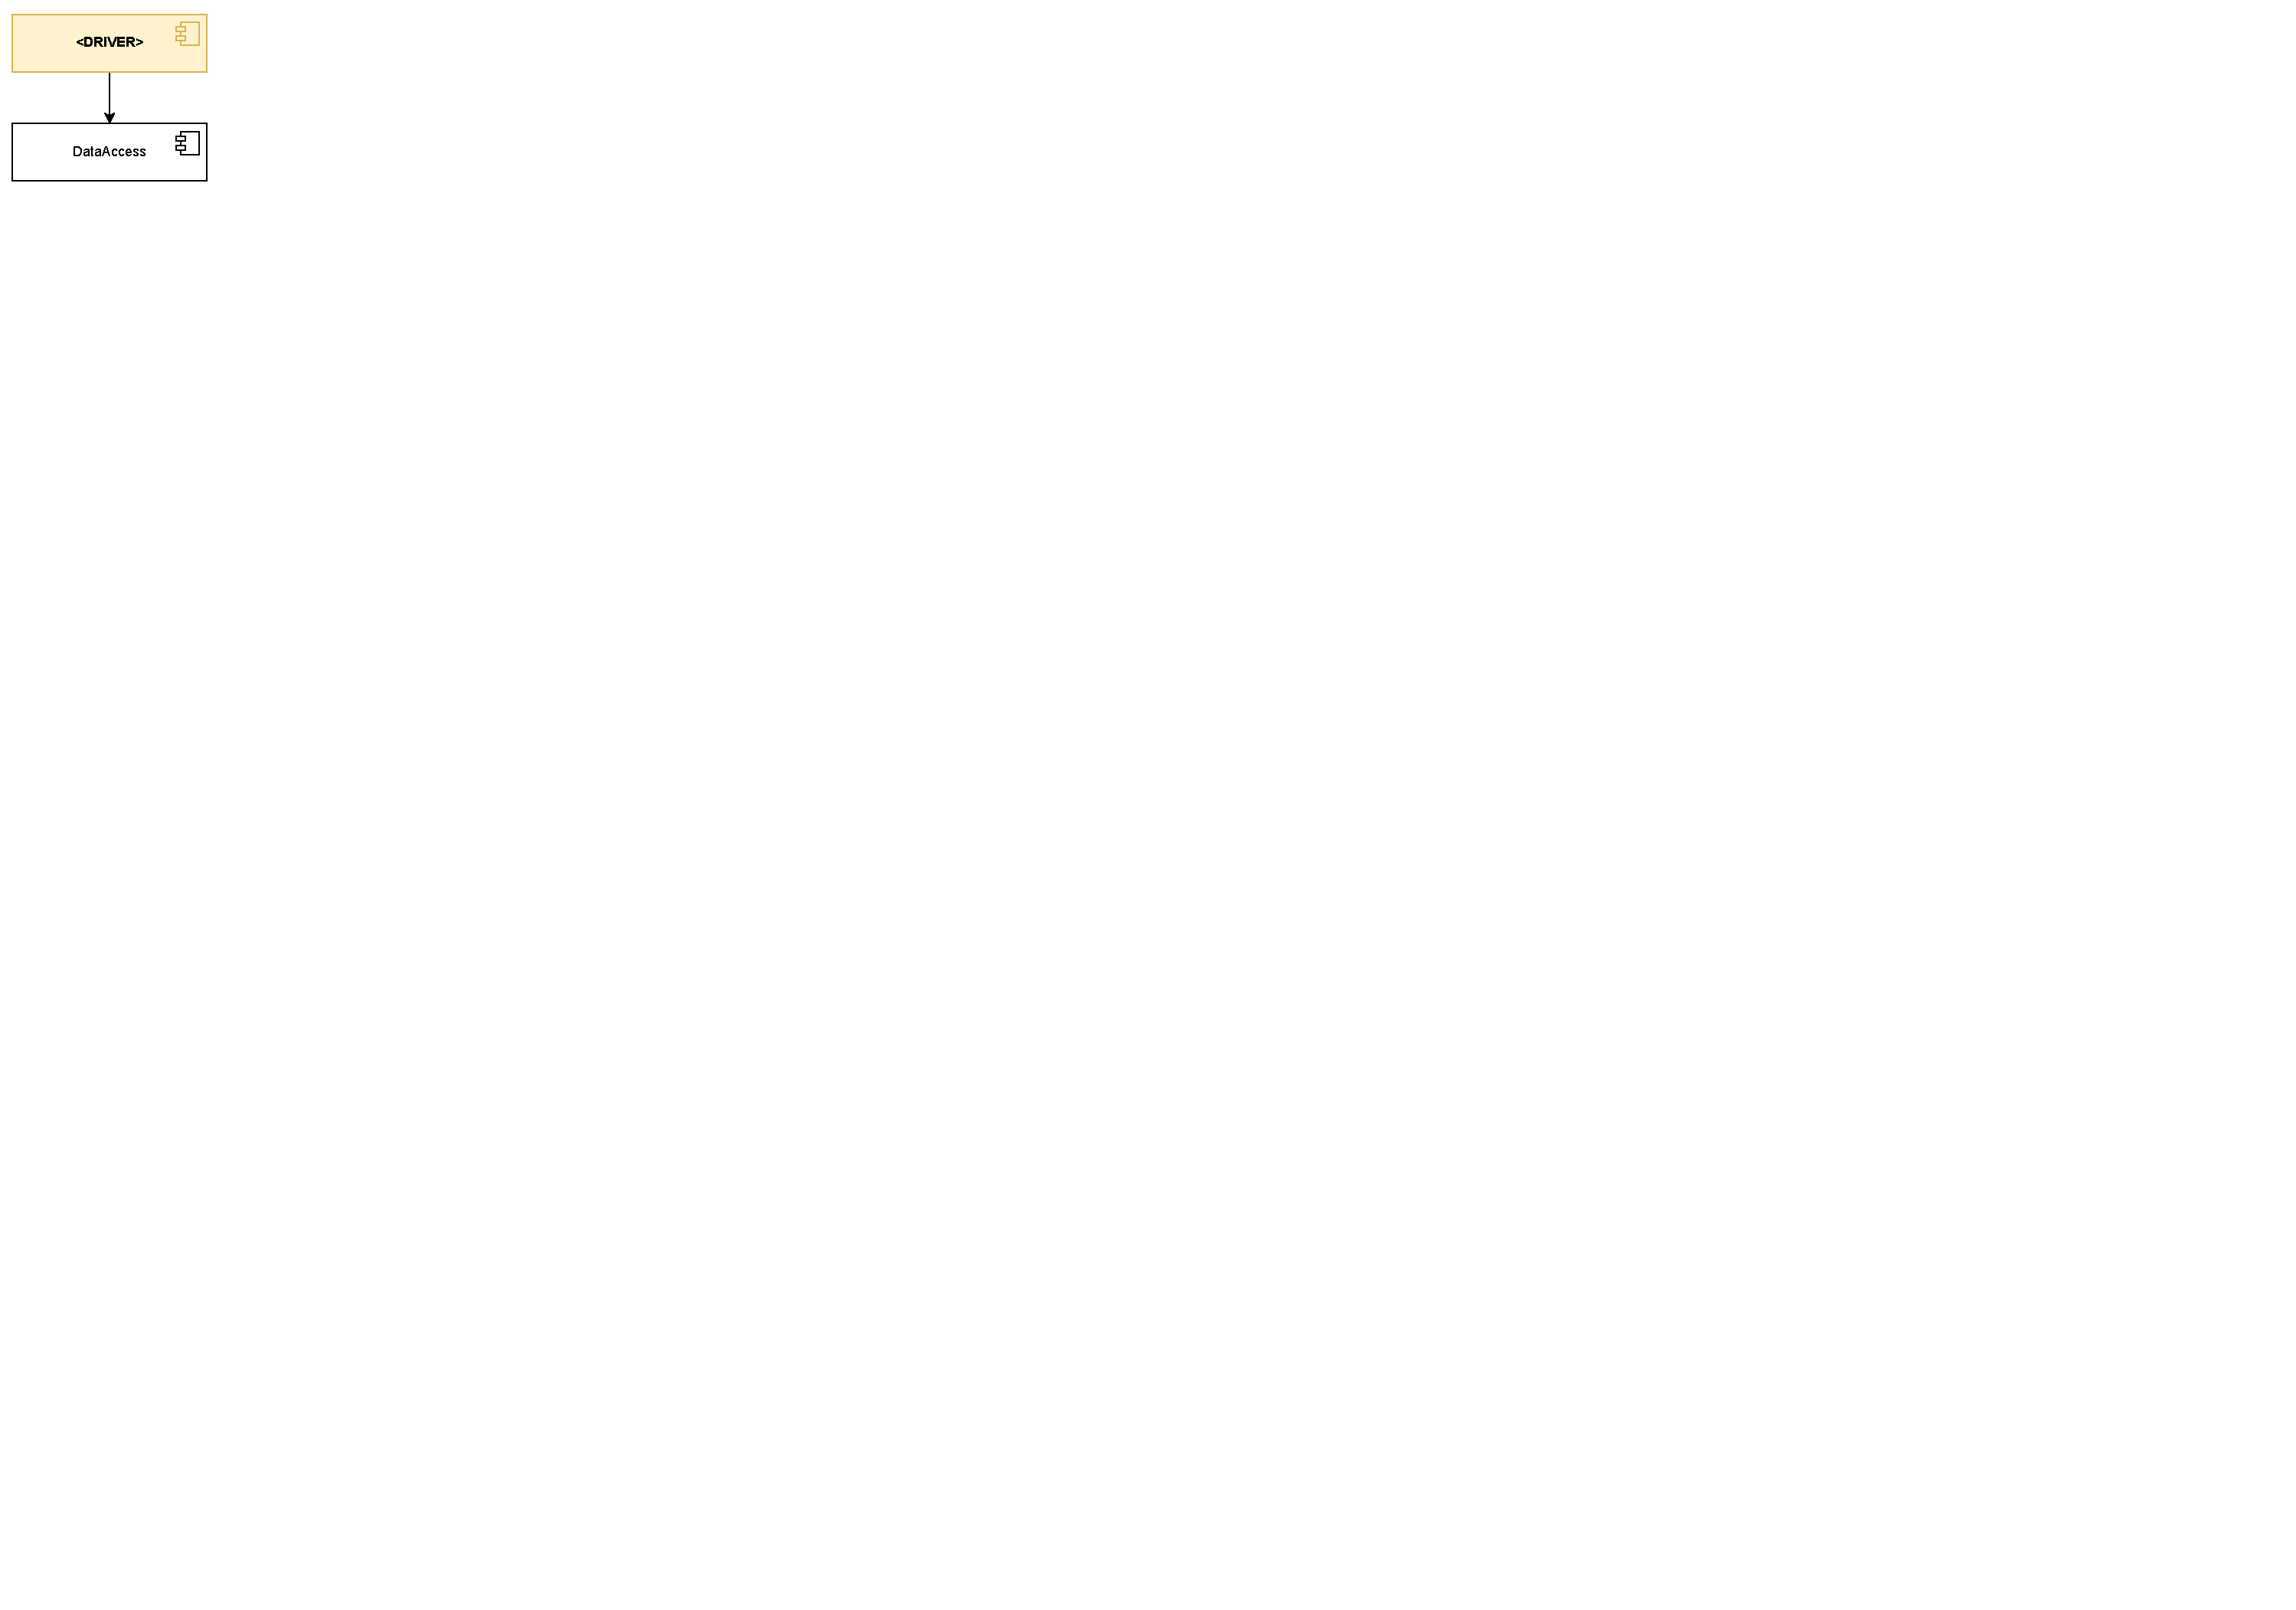
\includegraphics[page={1}, trim=0cm 31cm 46cm 0cmm, clip]{IntegrationDiagram.pdf}
    \caption{Data Access component integration}
\end{figure}

%trim = left bottom right top
\begin{figure}[!ht]
    \centering
    \includegraphics[page={2}, trim=0cm 31cm 46cm 0cmm, clip]{IntegrationDiagram.pdf}
    \caption{Payment Module component integration}
\end{figure}

\newpage

%trim = left bottom right top
\begin{figure}[!ht]
    \centering
    \includegraphics[page={3}, trim=0cm 27cm 26.5cm 0cmm, width=\linewidth, clip]{IntegrationDiagram.pdf}
    \caption{Bookings Manager, Recharge Manager, SearchCS, Register and Login components integration}
\end{figure}

%trim = left bottom right top
\begin{figure}[!ht]
    \centering
    \includegraphics[page={4}, trim=0cm 22.5cm 26.5cm 0cmm, width=\linewidth, clip]{IntegrationDiagram.pdf}
    \caption{Authentication and Request Router components integration}
\end{figure}

\newpage

%trim = left bottom right top
\begin{figure}[!ht]
    \centering
    \includegraphics[page={5}, trim=0cm 22.5cm 26.5cm 0cmm, width=\linewidth, clip]{IntegrationDiagram.pdf}
    \caption{Full integration}
\end{figure}

\subsubsection{CPMS Integration}

%trim = left bottom right top
\begin{figure}[!ht]
    \centering
    \includegraphics[page={6}, trim=0cm 31cm 46cm 0cmm, clip]{IntegrationDiagram.pdf}
    \caption{Data Access component integration}
\end{figure}

\newpage

%trim = left bottom right top
\begin{figure}[!ht]
    \centering
    \includegraphics[page={7}, trim=0cm 28.5cm 36.5cm 0cmm, width=0.7\linewidth, clip]{IntegrationDiagram.pdf}
    \caption{CS Manager component integration}
\end{figure}

%trim = left bottom right top
\begin{figure}[!ht]
    \centering
    \includegraphics[page={8}, trim=0cm 25.5cm 14cm 0cmm, width=\linewidth, clip]{IntegrationDiagram.pdf}
    \caption{DSO Information, Recharge Manger, CS List, Automatic Mode Manager, CS Prices Manager, CS DSO Manager, CS Battery Policy Manager and Login component integration}
\end{figure}

%trim = left bottom right top
\begin{figure}[!ht]
    \centering
    \includegraphics[page={9}, trim=0cm 21cm 14cm 0cmm, width=\linewidth, clip]{IntegrationDiagram.pdf}
    \caption{Authentication and Request Router component integration}
\end{figure}

\newpage

%trim = left bottom right top
\begin{figure}[!ht]
    \centering
    \includegraphics[page={10}, trim=0cm 21cm 14cm 0cmm, width=\linewidth, clip]{IntegrationDiagram.pdf}
    \caption{Full integration}
\end{figure}

\subsubsection{Whole System Integration}

%trim = left bottom right top
\begin{figure}[!ht]
    \centering
    \includegraphics[page={11}, trim=0cm 11cm 13cm 0cmm, width=\linewidth, clip]{IntegrationDiagram.pdf}
    \caption{eMSP and CPMS integration}
\end{figure}

\newpage

\section{Effort Spent}

\subsection{Ronzani Marco - mat: 224578}

\begin{tabular}{|l|l|}
    \hline
    \textbf{Task} & \textbf{Time spent} \\
    \hline
    Introduction & $\infty h$ \\
    \hline
    Architectural Design & $\infty h$ \\
    \hline
    User Interface Design & $\infty h$ \\
    \hline
    Requirements Traceability & $\infty h$ \\
    \hline
    Implementation, Integration and Test Plan & $\infty h$ \\
    \hline
    Other & $\infty h$ \\
    \hline
    \hline
    Total & $5*\infty h$ \\
    \hline
\end{tabular}

\subsection{Sassi Alessandro - mat: ...}

\begin{tabular}{|l|l|}
    \hline
    \textbf{Task} & \textbf{Time spent} \\
    \hline
    Introduction & $\infty h$ \\
    \hline
    Architectural Design & $\infty h$ \\
    \hline
    User Interface Design & $\infty h$ \\
    \hline
    Requirements Traceability & $\infty h$ \\
    \hline
    Implementation, Integration and Test Plan & $\infty h$ \\
    \hline
    Other & $\infty h$ \\
    \hline
    \hline
    Total & $5*\infty h$ \\
    \hline
\end{tabular}

\newpage

\section{References}
\label{section:references}

\begin{enumerate}
    \item \href{https://www.chargelab.co/}{ChargeLab - operating system for EV charges}
    \item \href{https://www.platformelectromobility.eu/2022/05/17/ev-charging-how-to-tap-in-the-grid-smartly/}{Platform for Electromobility. EV Charging: How to tap in the grid smartly?}.
    \item \href{https://mobilityintegrationsymposium.org/wp-content/uploads/sites/10/2018/11/4A_3_Emob18_024_paper_Filipe_Campos.pdf}{F. Campos, L. Marques, and K. Kotsalos, Electric Vehicle CPMS and Secondary Substation Management}.
    \item \href{https://doi.org/10.1145/3297067.3297078}{Shu Su, Hui Yan, and Ning Ding. 2018. Machine Learning-Based Charging Network Operation Service Platform Reservation Charging Service System. In Proceedings of the 2018 International Conference on Signal Processing and Machine Learning (SPML '18). Association for Computing Machinery, New York, NY, USA, 1–5}.
    \item Jan Mrkos, Antonín Komenda, and Michal Jakob. 2018. Revenue Maximization for Electric Vehicle Charging Service Providers Using Sequential Dynamic Pricing. In Proceedings of the 17th International Conference on Autonomous Agents and MultiAgent Systems (AAMAS '18). International Foundation for Autonomous Agents and Multiagent Systems, Richland, SC, 832–840.
\end{enumerate}
\end{document}
